\documentclass[specialist,
               substylefile = spbu_report.rtx,
               subf,href,colorlinks=true, 12pt]{disser}

\usepackage[a4paper,
            mag=1000, includefoot,
            left=3cm, right=1.5cm, top=2cm, bottom=2cm, headsep=1cm, footskip=1cm]{geometry}
\usepackage{mathtext}
\usepackage[T2A]{fontenc}
\usepackage[utf8]{inputenc}
\usepackage[english,russian]{babel}
\usepackage{amsmath}
\usepackage{amsthm}
\usepackage{bm}
\usepackage{bbold}
\usepackage{graphicx}
\usepackage{ textcomp }
\usepackage{subcaption}
\usepackage{longtable,booktabs,array}
\ifpdf\usepackage{epstopdf}\fi
\bibliographystyle{gost2008}

% Точка с запятой в качестве разделителя между номерами цитирований
%\setcitestyle{semicolon}

% Использовать полужирное начертание для векторов
\let\vec=\mathbf

% Включать подсекции в оглавление
\setcounter{tocdepth}{2}

\graphicspath{{fig/}}

\theoremstyle{definition}
\newtheorem{definition}{Определение}
\newtheorem{algorithm}{Алгоритм}
\newtheorem{remark}{Замечание}
\newtheorem{theorem}{Теорема}

%----------------------------------------------------------------
\usepackage{calc} % for calculating minipage widths
% Correct order of tables after \paragraph or \subparagraph
\usepackage{etoolbox}
\makeatletter
\patchcmd\longtable{\par}{\if@noskipsec\mbox{}\fi\par}{}{}
\makeatother
% Allow footnotes in longtable head/foot
\IfFileExists{footnotehyper.sty}{\usepackage{footnotehyper}}{\usepackage{footnote}}
\makesavenoteenv{longtable}

\usepackage{lmodern}
\usepackage{iftex}
\ifPDFTeX
  \usepackage[T1]{fontenc}
  \usepackage[utf8]{inputenc}
  \usepackage{textcomp} % provide euro and other symbols
\else % if luatex or xetex
  \usepackage{unicode-math}
  \defaultfontfeatures{Scale=MatchLowercase}
  \defaultfontfeatures[\rmfamily]{Ligatures=TeX,Scale=1}
\fi
% Use upquote if available, for straight quotes in verbatim environments
\IfFileExists{upquote.sty}{\usepackage{upquote}}{}
\IfFileExists{microtype.sty}{% use microtype if available
  \usepackage[]{microtype}
  \UseMicrotypeSet[protrusion]{basicmath} % disable protrusion for tt fonts
}{}
\makeatletter
\@ifundefined{KOMAClassName}{% if non-KOMA class
  \IfFileExists{parskip.sty}{%
    \usepackage{parskip}
  }{% else
    \setlength{\parindent}{0pt}
    \setlength{\parskip}{6pt plus 2pt minus 1pt}}
}{% if KOMA class
  \KOMAoptions{parskip=half}}
\makeatother
\usepackage{xcolor}
\IfFileExists{xurl.sty}{\usepackage{xurl}}{} % add URL line breaks if available
\IfFileExists{bookmark.sty}{\usepackage{bookmark}}{\usepackage{hyperref}}
\hypersetup{
  pdflang={ru-RU},
  hidelinks,
  pdfcreator={LaTeX via pandoc}}
\urlstyle{same} % disable monospaced font for URLs
\usepackage[margin=1in]{geometry}
\usepackage{color}
\usepackage{fancyvrb}
\newcommand{\VerbBar}{|}
\newcommand{\VERB}{\Verb[commandchars=\\\{\}]}
\DefineVerbatimEnvironment{Highlighting}{Verbatim}{commandchars=\\\{\}}
% Add ',fontsize=\small' for more characters per line
\usepackage{framed}
\definecolor{shadecolor}{RGB}{248,248,248}
\newenvironment{Shaded}{\begin{snugshade}}{\end{snugshade}}
\newcommand{\AlertTok}[1]{\textcolor[rgb]{0.94,0.16,0.16}{#1}}
\newcommand{\AnnotationTok}[1]{\textcolor[rgb]{0.56,0.35,0.01}{\textbf{\textit{#1}}}}
\newcommand{\AttributeTok}[1]{\textcolor[rgb]{0.77,0.63,0.00}{#1}}
\newcommand{\BaseNTok}[1]{\textcolor[rgb]{0.00,0.00,0.81}{#1}}
\newcommand{\BuiltInTok}[1]{#1}
\newcommand{\CharTok}[1]{\textcolor[rgb]{0.31,0.60,0.02}{#1}}
\newcommand{\CommentTok}[1]{\textcolor[rgb]{0.56,0.35,0.01}{\textit{#1}}}
\newcommand{\CommentVarTok}[1]{\textcolor[rgb]{0.56,0.35,0.01}{\textbf{\textit{#1}}}}
\newcommand{\ConstantTok}[1]{\textcolor[rgb]{0.00,0.00,0.00}{#1}}
\newcommand{\ControlFlowTok}[1]{\textcolor[rgb]{0.13,0.29,0.53}{\textbf{#1}}}
\newcommand{\DataTypeTok}[1]{\textcolor[rgb]{0.13,0.29,0.53}{#1}}
\newcommand{\DecValTok}[1]{\textcolor[rgb]{0.00,0.00,0.81}{#1}}
\newcommand{\DocumentationTok}[1]{\textcolor[rgb]{0.56,0.35,0.01}{\textbf{\textit{#1}}}}
\newcommand{\ErrorTok}[1]{\textcolor[rgb]{0.64,0.00,0.00}{\textbf{#1}}}
\newcommand{\ExtensionTok}[1]{#1}
\newcommand{\FloatTok}[1]{\textcolor[rgb]{0.00,0.00,0.81}{#1}}
\newcommand{\FunctionTok}[1]{\textcolor[rgb]{0.00,0.00,0.00}{#1}}
\newcommand{\ImportTok}[1]{#1}
\newcommand{\InformationTok}[1]{\textcolor[rgb]{0.56,0.35,0.01}{\textbf{\textit{#1}}}}
\newcommand{\KeywordTok}[1]{\textcolor[rgb]{0.13,0.29,0.53}{\textbf{#1}}}
\newcommand{\NormalTok}[1]{#1}
\newcommand{\OperatorTok}[1]{\textcolor[rgb]{0.81,0.36,0.00}{\textbf{#1}}}
\newcommand{\OtherTok}[1]{\textcolor[rgb]{0.56,0.35,0.01}{#1}}
\newcommand{\PreprocessorTok}[1]{\textcolor[rgb]{0.56,0.35,0.01}{\textit{#1}}}
\newcommand{\RegionMarkerTok}[1]{#1}
\newcommand{\SpecialCharTok}[1]{\textcolor[rgb]{0.00,0.00,0.00}{#1}}
\newcommand{\SpecialStringTok}[1]{\textcolor[rgb]{0.31,0.60,0.02}{#1}}
\newcommand{\StringTok}[1]{\textcolor[rgb]{0.31,0.60,0.02}{#1}}
\newcommand{\VariableTok}[1]{\textcolor[rgb]{0.00,0.00,0.00}{#1}}
\newcommand{\VerbatimStringTok}[1]{\textcolor[rgb]{0.31,0.60,0.02}{#1}}
\newcommand{\WarningTok}[1]{\textcolor[rgb]{0.56,0.35,0.01}{\textbf{\textit{#1}}}}
\usepackage{graphicx}
\makeatletter
\def\maxwidth{\ifdim\Gin@nat@width>\linewidth\linewidth\else\Gin@nat@width\fi}
\def\maxheight{\ifdim\Gin@nat@height>\textheight\textheight\else\Gin@nat@height\fi}
\makeatother
% Scale images if necessary, so that they will not overflow the page
% margins by default, and it is still possible to overwrite the defaults
% using explicit options in \includegraphics[width, height, ...]{}
\setkeys{Gin}{width=\maxwidth,height=\maxheight,keepaspectratio}
% Set default figure placement to htbp
\makeatletter
\def\fps@figure{htbp}
\makeatother
\setlength{\emergencystretch}{3em} % prevent overfull lines
\providecommand{\tightlist}{%
  \setlength{\itemsep}{0pt}\setlength{\parskip}{0pt}}
\setcounter{secnumdepth}{-\maxdimen} % remove section numbering
\ifLuaTeX
\usepackage[bidi=basic]{babel}
\else
\usepackage[bidi=default]{babel}
\fi
\babelprovide[main,import]{russian}
% get rid of language-specific shorthands (see #6817):
\let\LanguageShortHands\languageshorthands
\def\languageshorthands#1{}
\ifLuaTeX
  \usepackage{selnolig}  % disable illegal ligatures
\fi

%-------------------------------
\begin{document}

%
% Титульный лист на русском языке
%
% Название организации
\institution{%
    Санкт-Петербургский государственный университет\\
    Прикладная математика и информатика
}

\title{Отчет по научно-исследовательской работе}

% Тема
\topic{Улучшение разделимости для автоматизации метода SSA}

% Автор
\author{Дудник Павел Дмитриевич}
\group{группа 19.Б04-мм}
    
% Научный руководитель
\sa       {Голяндина Нина Эдуардовна\\%
           Кафедра Статистического Моделирования}
\sastatus {к.\,ф.-м.\,н., доцент}

% Город и год
\city{Санкт-Петербург}
\date{\number\year}

\maketitle

\tableofcontents

\intro
В задачах, использующих временные ряды, часто требуется знать структуру этих рядов, разложение в сумму интерпретируемых компонент, например, для того, чтобы прогнозировать значения или заполнять пропуски. Такое разложение позволяет получить метод SSA, имеющий множество применений и описанный, например, в пособии \cite{Golyandina04}. Однако применение этого метода осложняется тем, что получение результата не является полностью автоматическим и требует визуального анализа. Также существует проблема отсутствия слабой/сильной разделимости компонент временного ряда, что не позволяет применить метод SSA. Существование этих проблем служит мотивацией для написания этой работы и проведения экспериментов.

В данной работе рассматривается проблема улучшения разделимости для автоматизации разложения временного ряда в сумму компонент, была поставлена задача создания алгоритма/нескольких алгоритмов для решения этой проблемы. Иначе говоря, алгоритм должен автоматически получать разложение в условиях недостатка разделимости компонент. В качестве базового метода, позволяющего извлечь компоненты, используется метод SSA.

В работе были предложены решения, позволяющие получить разделимость компонент временного ряда и произвести автоматическую группировку компонент, при этом решения используют модификации алгоритма SSA - IOSSA (Iterative Oblique SSA) и EOSSA (ESPRIT-based Oblique SSA). Описание необходимых для описания решений результатов (методов, определений и теорем) находится в разделе 1.

Первая часть работы посвящена решениям, использующих метод IOSSA для автоматического выделения тренда, проведено сравнение решений и наиболее точного метода для этой задачи - ручной группировки компонент. Программа с экспериментами и сравнением решений находится в приложении к работе.

Вторая часть посвящена проблеме обобщения алгоритма EOSSA на случай кратных сигнальных корней.

\chapter{Вспомогательные результаты}
\section{Модель временного ряда}
\begin{definition}
    ~$F_N = (f_1, \ldots, f_N)$ --- \textbf{временной ряд} длины $N$, $f_i \in \mathbb{R}$ --- наблюдение в момент времени $i$.
    
    $F_N = F_{Signal} + F_{Noise}$, $F_{Signal} = F_{Trend} + F_{Residuals}$ --- детерминированная составляющая; $F_{Trend}, F_{Residuals}, F_{Noise}$ --- временные ряды длины N, компоненты ряда $F$.
    \begin{itemize}
        \item $F_{Trend}$ --- тренд, медленно меняющаяся компонента
        \item $F_{Residuals}$ --- остаток, сумма периодических компонент
        \item $F_{Noise}$ --- шум, случайная составляющая
    \end{itemize}
\end{definition}
\section{Метод <<Гусеница>>-SSA}
\begin{algorithm}
    ~Пусть $F_N=(f_1, \ldots, f_N)$ --- временной ряд, N --- его длина. $1<L<N$ --- длина окна.
    \begin{enumerate}
	    \item \textbf{Вложение}: $K=N-L+1$, ряд переводится в траекторную матрицу $\bm{X}=[X_1:\ldots:X_K]$, где $X_i = (f_i, \ldots, f_{i + L - 1})^{\mathrm{T}}$, $1 \leq i \leq K$.

	    \item Строится сингулярное разложение траекторной матрицы: $\bm{X} = \sum\limits_{i=1}^d \sqrt{\lambda_i}U_iV_i^{\mathrm{T}} = \sum\limits_{i=1}^d\bm{X}_i$, $1 \leq i \leq d = rank\bm{X}$, $\sqrt{\lambda_i}$ --- сингулярные числа, $\bm{X}_i$ --- траекторная матрица элементарной компоненты (временного ряда, который соответствует одному слагаемому в сингулярном разложении).

	    \item \textbf{Группировка}: $\bm{X} =  \sum\limits_{i=1}^r \widetilde{\bm{X}_i}$, где $\widetilde{\bm{X}_i}$ --- траекторная матрица компоненты, состоящей из одной или нескольких элементарных компонент, r --- число компонент.

	    \item \textbf{Диагонализация}: каждая траекторная матрица компоненты переводится во временной ряд с помощью диагонального усреднения.
	\end{enumerate} 
	Более подробно алгоритм изложен в пособии \cite{Golyandina04}.
\end{algorithm}
\section{Разложение Фурье}
\begin{definition}
    ~Пусть $F_N=(f_1, \ldots, f_N)$ --- временной ряд, N --- его длина. Разложение Фурье для временного ряда:
    \begin{equation*} \label{eq2} \tag{2}
        f_n = c_0 + \sum\limits_{k = 1}^{\lfloor \frac{N - 1}{2}\rfloor} \sqrt{c_k^2 + s_k^2}\mathsf{cos}(\frac{2\pi nk}{N} + \phi_k) + c_{\frac{N}{2}}(-1)^k.
    \end{equation*}
\end{definition}
\begin{definition}
    ~Пусть имеется разложение \eqref{eq2}. Тогда следующая функция называется периодограммой:
    \begin{equation*}
                \Pi^f_N (\frac{k}{N}) = \frac{N}{2}
        \begin{cases}
        2c_0^2 & ,k = 0\\
        c_k^2+s_k^2 & ,0 < k < N/2\\
        2c^2_{N/2} & ,k = N/2
        \end{cases}
    \end{equation*}
\end{definition}
    
\begin{definition}
    ~Частота $\omega$ является низкой, если она меньше некоторой $\omega_0 > 0$. Вклад низких частот в ряд --- это $\sum\limits_{0 \leq \frac{k}{N} < \omega_0}\Pi_N^f(\frac{k}{N})$.
\end{definition}

\section{Oblique SSA}

\begin{definition}
    Пусть $X, Y \in \mathbb{R}^n, \mathbf{A} \in \mathbb{R}^{n \times n}$. Векторы $X, Y$ называются $\mathbf{A}$-ортогональными, если
    \begin{equation*}
        (\mathbf{A}X, Y) =  \langle X, Y\rangle _{\mathbf{A}}.
    \end{equation*}
\end{definition}
\begin{definition}
    Будем говорить, что пара матриц $(\mathbf{L}, \mathbf{R})$ согласованы с матрицей $\mathbf{X}$, если пространство столбцов $\mathbf{L}$ содержит пространство столбцов $\mathbf{X}$ и пространство столбцов $\mathbf{R}$ содержит пространство строк $\mathbf{X}$.
\end{definition}
\begin{definition}
    Пусть пара матриц $(\mathbf{L}, \mathbf{R})$ согласованна с $\mathbf{X}$. Тогда минимальное разложение ранга $r$
    \begin{equation*}
        \mathbf{X} = \sum_{i = 1}^{r}\sigma_iP_iQ_i^{\mathrm{T}}
    \end{equation*}\\
    будем называть $(\mathbf{L}, \mathbf{R})$-SVD ( $(\mathbf{L}, \mathbf{R})$-сингулярным разложением) матрицы $\mathbf{X}$.
\end{definition}

Алгоритм построения $(\mathbf{L}, \mathbf{R})$-SVD подробно описан в разделе 3 статьи \cite{Golyandina15}.

\begin{definition}
    Пусть длина окна $L$ фиксирована. Ряды $\mathbb{X}^{(1)}$ и $\mathbb{X}^{(2)}$ называются слабо $(\mathbf{L}, \mathbf{R})$-разделимыми, если их траекторные пространства столбцов $\mathbf{L}$-ортогональны и траекторные пространства строк $\mathbf{R}$-ортогональны между собой, т.е.
    \begin{equation*}
        (\mathbf{X}^{(1)})^{\mathrm{T}}\mathbf{LX}^{(2)} = 0_{K \times K}, (\mathbf{X}^{(1)})\mathbf{R}(\mathbf{X}^{(2)})^{\mathrm{T}} = 0_{L \times L}.
    \end{equation*}

\end{definition}
    
\begin{definition}
    Ряды $\mathbb{X}^{(1)}$ и $\mathbb{X}^{(2)}$ называются сильно $(\mathbf{L}, \mathbf{R})$-разделимыми, если они слабо $(\mathbf{L}, \mathbf{R})$-разделимы и при этом наборы сингулярных чисел из SVD траекторных матриц $\mathbf{X}^{(1)}$ и $\mathbf{X}^{(2)}$ не пересекаются.
\end{definition}


\subsection{Nested Oblique SSA}
\begin{algorithm}
    В условиях раздела 1.2:
\end{algorithm}
Пусть даны траекторная матрица $\mathbf{X}$ и согласованные с ней $\mathbf{L}, \mathbf{R}$.
    \begin{enumerate}
        \item Строится $(\mathbf{L}, \mathbf{R})$-SVD матрицы $\mathbf{X}$.
        \item Группируются траекторные матрицы элементарных компонент.
        \item Производится диагональное усреднение траекторных матриц.
    \end{enumerate}
    Таким образом, результат алгоритма - разложение временного ряда, соответствующего траекторной матрице $\mathbf{X}$.
    \begin{remark}
    Nested Oblique SSA не может быть применен для реальных задач, так как матрицы $\mathbf{L}, \mathbf{R}$ определяются траекторными пространствами компонент, которые мы хотим получить в разложении, при этом эти пространства неизвестны, так как мы не обладаем знаниями о компонентах.
    \end{remark}
\subsection{Iterative Oblique SSA}
    IOSSA (Iterative Oblique SSA) --- это итеративная модификация Nested OSSA. 
    
    Пусть имеется траекторная матрица $\mathbf{X}$, пара матриц $(\mathbf{L}^{(0)}, \mathbf{R}^{(0)})$ инициализированная единичными матрицами и некоторое разбиение множества индексов $\{ 1,...,r\}$, где r - ранг минимального разложения матрицы $\mathbf{X}$, тогда $(\mathbf{L}^{(0)}, \mathbf{R}^{(0)})$-SVD матрицы $\mathbf{X}$ это обычное сингулярное разложение.
    \begin{algorithm}
        На шаге $k \geq 1$:
        \begin{enumerate}
            \item Вычисляются $(\mathbf{L}^{(k)}, \mathbf{R}^{(k)})$ согласованные с $\mathbf{X}$ (используются траекторные пространства рядов, полученных в результате группировке предыдущего $(\mathbf{L}^{(k - 1)}, \mathbf{R}^{(k - 1)})$-SVD согласно разбиению множества индексов).
            \item Строится $(\mathbf{L}^{(k)}, \mathbf{R}^{(k)})$-SVD матрицы $\mathbf{X}$.
            \item Производится группировка согласно разбиению и диагональное усреднение, тем самым, получаем разложение ряда $\mathbb{X}$.
        \end{enumerate}
        Шаги повторяются до сходимости компонент.
    \end{algorithm}
    \begin{remark}
        Модификация алгоритма IOSSA, называемая модификацией с $\sigma$-коррекцией, описаная в подразделе 3.3.2 статьи \cite{Golyandina15} позволяет изменять разбиение индексов (это позволяет, например, избежать проблем при неудачном начальном разбиении) и ослабляет условия сильной разделимости. В разделе 2 используется именно эта модификация.
    \end{remark}
    
    \subsection{ESPRIT-motivated Oblique SSA}
    Будем рассматривать ряды конечной размерности, описанные в статье \cite{Shlemov}.
    \begin{definition}
        Ряд $\mathbb{S} = (s_1, .., s_N)$ управлется линейной рекуррентной формулой (ЛРФ), если
        \begin{equation*}
            s_{r+i} = a_1s_{r+i - 1} + a_2s_{r+i - 2} + . . . + a_rs_i
, \forall i \in 1, . . . , N - r.
        \end{equation*}
        При этом $r$ называется порядком ЛРФ.
    \end{definition}
    Для любого ряда, управляемого ЛРФ существует единственная ЛРФ минимального порядка.
    При этом если все корни характеристического полинома $\chi_{\mathbf{a}} (\mu ) = \mu^r - \sum^r_{k=1} a_k\mu^{r - k}$ различны, то элементы ряда $\mathbb{S}$ могут быть представлены в виде:
    \begin{equation*}
        s_j =\sum^r_{k=1} Ak\mu^j_k
, A_k \in \mathbb{C}.
    \end{equation*}
    Таким образом, ряд конечной размерности представим в виде
суммы экспонент (соответствующих вещественным корням характеристического полинома) и
экспоненциально-модулированных гармоник (соответствующих парам
комплексно-сопряженных корней характеристического полинома).

Метод EOSSA (ESPRIT-based Oblique SSA) использует метод ESPRIT, описанный в статье \cite{Roy89}, чтобы разделять компоненты в случае недостатка разделимости компонент.

В случае различных сигнальных корней можно применить следующую теорему:

\begin{theorem}
\label{th1}
Пусть ряд $\mathbb{S}$ длины $N$ --— ряд конечной размерности r и все сигнальные корни характеристического полинома минимальной управляющей ЛРФ различны, $L > r$, $K = N - L + 1 > r$, $\mathbf{S} = \mathcal{T}_L\mathbb{S}$ --— $L$-траекторная матрица. Пусть $\mathbf{S} = \mathbf{P Q}^{\mathrm{T}}$ --— минимальное комплексное разложение матрицы $\mathbf{S}$, т.е. $\mathbf{P} \in \mathbb{R}^{L \times r}$, $\mathbf{Q} \in \mathbb{R}^{K \times r}$. \\
    \hspace*{0.5cm} Тогда:
    \begin{enumerate}
        \item Матрица $\mathbf{P}$ обладает сдвиговым свойством: $\overline{\mathbf{P}} = \underline{\mathbf{P}}\mathbf{M}$ для некоторой матрицы $\mathbf{M} \in \mathbb{R}^{r \times r}$.
        \item Собственные числа матрицы $\mathbf{M}$ совпадают с корнями х.п. $\mu_k$ и их кратностями.
        \item Пусть $\mathbf{M} = \mathbf{T}diag(\mu_1, ..., \mu_r)\mathbf{T}^{-1}, \mathbf{T} \in \mathbb{C}^{r \times r}$ - спектральное разложение матрицы $\mathbf{M}$.
        Тогда $\mathbf{S} = \mathbf{\Pi \Psi}^{\mathrm{T}} = (\mathbf{PT})(\mathbf{T}^{-1}\mathbf{ Q}^{\mathrm{T}}), \mathbf{\Pi} \in \mathbb{C}^{L \times r}, \mathbf{\Psi} \in \mathbb{C}^{K \times r}$, где $\mathbf{\Pi} = \mathbf{PT}$ и $\mathbf{\Psi}^{\mathrm{T}} = \mathbf{T}^{-1}\mathbf{Q}^{\mathrm{T}}$, причем:
        \begin{itemize}
            \item $\mathbf{\Pi} = [\Pi_1: \ldots :\Pi_r], \mathbf{\Pi}_k \in \mathbb{C}^{L}$ соответствует k-ому сигнальному корню ; Матрица $\mathbf{\Pi}$ имеет Вандермондовскую структуру: $\Pi_k \propto (\mu_k, \mu_k^2, ..., \mu_k^L)$.
            
            \item $\mathbf{\Psi} = [\Psi_1: \ldots :\Psi_r], \mathbf{\Psi}_k \in \mathbb{C}^{K}$ соответствует k-ому сигнальному корню; Матрица $\mathbf{\Psi}$ имеет Вандермондовскую структуру: $\Psi_k \propto (\mu_k, \mu_k^2, ..., \mu_k^K)$.
        \end{itemize}
    \end{enumerate}

\end{theorem}
Таким образом, получаем разложение траекторной матрицы $\mathbf{S} = \sum^r_{k=1} \Pi_k\Psi_k^{\mathrm{T}} = \mathbf{\Pi \Psi}^{\mathrm{T}}$. Это приводит к следующему алгоритму (EOSSA):
\begin{algorithm} В условиях предыдущей теоремы:
\label{alg4}
    \begin{enumerate}
            \item Получаем минимальное разложение траекторной матрицы сигнала $\mathbf{S} = \mathbf{PQ}^{\mathrm{T}}$
            \item Оцениваем сдвиговую матрицу $\mathbf{M}$.
            \item Строим спектральное разложение сдвиговой матрицы $\mathbf{M} = \mathbf{T}diag(\mu_1, ..., \mu_r)\mathbf{T}^{-1}$.
            \item Строим разложение $\mathbf{S} = (\mathbf{PT})(\mathbf{T}^{-1}\mathbf{Q}^{\mathrm{T}}) = \mathbf{\Pi \Psi}^{\mathrm{T}} = \sum_{k = 1}^{r}\mathbf{\Pi}_k\mathbf{\Psi}^{\mathrm{T}}_k$.
            \item Производим группировку попарно сопряженных компонент.
            \item Восстановление компонент через диагональное усреднение. 
        \end{enumerate}
\end{algorithm}
Более подробно алгоритм изложен в работе \cite{Shlemov}.
    \label{algorithm:4}
    \begin{definition}
        Функция
        \begin{equation*}
            F_m[X] = \begin{cases}
            0, & m < 0 \\
            1, & m = 0 \\
            \frac{1}{m!}\prod_{i=0}^{m - 1}(X - i), & m>0
            \end{cases}
        \end{equation*}
        называется убывающим факториалом.
    \end{definition}
    
    
    
    
\chapter{Автоматизация выделения тренда с помощью алгоритма IOSSA}
\section{Формализация задачи}
Пусть имеется небольшое $\omega_0 > 0$ и $0 < T < 1$ близкое к единице, тогда будем относить к тренду компоненту временного ряда, у которой вклад низких частот больше $T$ (такой вклад назовем большим):
\begin{equation*}
    \sum\limits_{0 \leq \frac{k}{N} < \omega_0}\Pi_N^f(\frac{k}{N}) > T.
\end{equation*}

Таким образом, имея разложение ряда, например, полученное с помощью базового SSA, можно отобрать элементарные компоненты таким способом, получив тренд.

Однако при отсутствии разделимости компонент нельзя автоматически выделить тренд, поэтому можно ослабить условие ортогональности. Для этого в решениях используется алгоритм IOSSA.

В обоих решениях сначала выбирается длина окна $L$ и число компонент в сигнале $r$, применяется базовый алгоритм SSA и $r$ первых слагаемых в сингулярном разложении отбираются в траекторную матрицу сигнала. Таким образом, компоненты, соответствующие шуму, просто помещаются в остаток.
\section{Придуманные решения}
\subsection{Решение с автоматической группировкой}
Пусть имеется временной ряд $\mathbb{X}$. Выберем длину окна, а также количество компонент в сигнале.

В этом решении в качестве начальной группировки в одну группу помещаются элементарные компоненты сигнала с большим вкладом низких частот, в другую — остальные. Далее применяется IOSSA. В результате получаем тренд, компоненту с периодиками и остаток.

\subsection{Решение без группировки}
В этом решении в качестве начальной группировки каждая элементарная компонента сигнала помещается в отдельную группу. Далее применяется IOSSA, результат выполнения --- $r$ компонент из одной элементарной компоненты.

После этого относим к тренду компоненты с большим вкладом низких
частот. В результате получаем тренд, компоненту с периодиками и остаток.

\section{Эксперименты}
\subsection{Эксперимент 1}
В эксперименте был создан временной ряд $f_n , 0\leq n < N, N=101$, с функцией тренда $0.08e^{0.01n}$, гармониками $0.25 * \mathsf{cos}(\frac{\pi n}{4} + \frac{\pi}{4})$ и $0.25 * \mathsf{cos}(\frac{2 \pi n}{3})$, добавлен стандартный гауссовский шум $0.2 \varepsilon_n$.
Сравнивались автоматическое выделение тренда без применения IOSSA и решение без группировки.

Эксперимент показал, что при автоматическом выделении тренда без применения IOSSA тренд смешался с гармониками, при этом решение без группировки достаточно точно выделило тренд. Более подробно результаты эксперимента изложены в приложении А.

\subsection{Эксперимент 2}
В эксперименте был создан временной ряд $f_n , 0\leq n < N, N=101$, с функцией тренда $0.001n^2-0.5n+3$ и гармоникой $4.02 * \mathsf{cos}(\frac{2\pi n}{3})$, добавлен стандартный гауссовский шум $2 \varepsilon_n$.
Сравнивались автоматическое выделение тренда без применения IOSSA и решение без группировки.

Эксперимент показал, что при автоматическом выделении тренда без применения IOSSA тренд смешался с гармониками, при этом решение без группировки достаточно точно выделило тренд. Более подробно результаты эксперимента изложены в приложении А.

\subsection{Эксперимент 3}
В эксперименте был создан временной ряд $f_n , 0\leq n < N, N=101$, с функцией тренда $0.001n^2-0.5n+3$ и гармоникой $4.02 * \mathsf{cos}(\frac{2\pi n}{3})$, добавлен стандартный гауссовский шум $2 \varepsilon_n$.
Сравнивались алгоритм с автоматическим выделением тренда после фиксированной группировки и решение без группировки.

\begin{table}[h]
\caption{Среднеквадратическая ошибка извлечения тренда}
\label{tabular:1}
\begin{center}
\begin{tabular}{|c | c|}
\hline
 & MSE \\
\hline
Алгоритм с фикс. группировкой &  0.2233865\\
Решение без группировки & 0.2287474 \\
\hline
\end{tabular}
\end{center}
\end{table}
Решение без группировки показало сравнительно хорошую точность (см. Таблицу \ref{tabular:1}) в сравнении с алгоритмом с фиксированной группировкой.

\begin{remark}
    Алгоритм с автоматическим выделением тренда после фиксированной группировки применим в этом эксперименте, так как известно количество элементарных компонент в тренде в этом примере.
\end{remark}
\subsection{Эксперимент 4}
В эксперименте был создан временной ряд $f_n , 0\leq n < N, N=101$, с функцией тренда $2e^{0.03n} - 0.1n - 20$ и гармониками $5.2\mathsf{cos}(\frac{2\pi n}{6} + \frac{\pi}{4})$, $5.2\mathsf{cos}(\frac{2 \pi n} {3})$, добавлен стандартный гауссовский шум $0.2 \varepsilon_n$.
Сравнивались алгоритм с фиксированной группировкой (которая была найдена с помощью визуального анализа графика собственных векторов), решение с автоматической группировкой, а также решение без группировки. Решения сравнивались с методом с фиксированной группировкой и между собой. Моделирование ряда производилось 100 раз для оценки устойчивости методов.

Согласно результатам, полученным в результате эксперимента (результаты отражены в Таблице \ref{tabular:2}), решению без группировки требуется большое количество итераций до сходимости (в среднем 477 итерации). При этом можно увидеть, что медианное количество итераций значительно меньше среднего, что говорит о некотором количестве случаев сходимость затруднялась. Ошибка выделения тренда сравнима с методом с фиксированной группировкой.

Решение с автоматической группировкой показало большую среднюю ошибку выделения тренда (на порядок больше, чем у других методов), при этом медианная ошибка сравнима с медианными ошибками остальных двух методов. Это говорит о том, что в нескольких случаях автоматическая группировка была произведена неверно. Количество итераций при этом примерно такое же, как у метода с фиксированной группировкой.

Так же в результатах вычислялась средняя и медианная ошибка выделения остатка (периодических компонент), эти значения примерно соответствуют средней и медианной ошибке выделения тренда.

Этот эксперимент позволил составить рекомендации по применению определенного решения:
\begin{enumerate}
    \item Решение с автоматической группировкой лучше применять, когда нужно быстро вычислять разложение и при этом не требуется всегда точного результата (допускается некоторая доля неудачных разложений).
    \item Решение без группировки лучше применять, когда точность важна и при этом не нужна большая скорость вычислений (среднее количество итераций больше на два порядка, чем у другого решения).
\end{enumerate}

\begin{table}[h]
\footnotesize
\caption{Сравнение трех методов}
\label{tabular:2}
\begin{center}
\begin{tabular}{|c | c| c| c|}
\hline
 & MSE, выделение тренда & MSE, выделение остатка & Количество итераций \\
\hline
no grouping & mean: 0.0031, med: 0.003 & mean: 0.0054, med: 0.005 &
mean: 477, med: 372 \\
manual grouping & mean: 0.0019, med: 0.0016 & mean: 0.0044, med: 0.0041
& mean: 4, med: 4 \\
auto grouping & mean: 0.3337, med: 0.0017 & mean: 0.3268, med: 0.0044 &
mean: 5, med: 4 \\
\hline
\end{tabular}
\end{center}
\end{table}

\chapter{Обобщение алгоритма EOSSA на случай кратных сигнальных корней}
Для задачи, поставленной в начале, можно использовать алгоритм EOSSA (Алгоритм \ref{alg4}). Однако существует необходимость в обобщении EOSSA на случай кратных сигнальных корней. Для этого сначала приведем подробное доказательство Теоремы \ref{th1}:

\begin{theorem}
Пусть ряд $\mathbb{S}$ длины $N$ — ряд конечной размерности r и все
корни $\{ \mu_k\}_{k=1}^r$ характеристического полинома минимальной управляющей ЛРФ различны, $L > r$, $K = N - L + 1 > r$, $\mathbf{S} = \mathcal{T}_L\mathbb{S}$ — $L$-траекторная матрица. Пусть $\mathbf{S} = \mathbf{PQ}^{\mathrm{T}}$ — минимальное разложение матрицы $\mathbf{S}$, т.е. $\mathbf{P} \in \mathbb{R}^{L \times r}$ и $\mathbf{Q} \in \mathbb{R}^{K \times r}$. \\
    \hspace*{0.5cm} Тогда:
    \begin{enumerate}
        \item Матрица $\mathbf{P}$ обладает сдвиговым свойством: $\overline{\mathbf{P}} = \underline{\mathbf{P}}\mathbf{M}$ для некоторой матрицы $\mathbf{M} \in \mathbb{R}^{r \times r}$.
        \item Собственные числа матрицы $\mathbf{M}$ совпадают с корнями х.п. $\mu_k$.
        \item Пусть $\mathbf{M} = \mathbf{T}$diag$(\mu_1,\dots,\mu_r)\mathbf{T}^{-1}, \mathbf{T} \in \mathbb{C}^{r \times r}$ - спектральное разложение (eigen\-decomposition, EVD) матрицы $\mathbf{M}$.Тогда $\mathbf{S} = \mathbf{\Pi\Psi}^{\mathrm{T}} = (\mathbf{PT})(\mathbf{Q}(\mathbf{T}^{-1})^{\mathrm{T}})^{\mathrm{T}}, \mathbf{\Pi} \in \mathbb{C}^{L \times r}, $\\$\mathbf{\Psi} \in \mathbb{C}^{K \times r}$ - комплексное минимальное разложение матрицы $\mathbf{S}$, где матрицы $\mathbf{\Pi} = \mathbf{PT}$ и $\mathbf{\Psi} = \mathbf{Q}(\mathbf{T}^{-1})^{\mathrm{T}}$ имеют Вандермондовскую структуру: $\mathbf{\Pi} = [\Pi_1: \ldots :\Pi_r], \mathbf{\Psi} = [\Psi_1: \ldots :\Psi_r]$, где $\Pi_k \propto(\mu_k,\mu_k^2, \dots, \mu_k^L)^{\mathrm{T}}, \Psi_k \propto(1,\mu_k, \dots, \mu_k^{K - 1})^{\mathrm{T}}$.
    \end{enumerate}

\end{theorem}
\begin{proof}
Доказательство первых двух пунктов теоремы приведено в работе \cite{Huffel94}.

Доказательство п. 3. Рассмотрим разложение ряда $\mathbb{S}$ в сумму компонент в форме $s_j = \sum_{k = 1}^{r}A_k\mu_k^j$, $A_k \in \mathbb{C}$. Оно соответствует разложению траекторной матрицы $\mathbf{S} = \sum_{k = 1}^{r}\Pi_k\Psi_k^{\mathrm{T}} = \mathbf{\Pi\Psi}^{\mathrm{T}}$. Рассмотрим матрицу $\mathbf{T} \in \mathbb{C}^{r \times r}$ такую, что $\mathbf{\Pi} = \mathbf{PT}$. Такая $\mathbf{T}$ всегда существует и единственна, т.к. $\mathbf{PQ}^{\mathrm{T}} = \mathbf{\Pi\Psi}^{\mathrm{T}}$ - минимальные разложения матрицы $\mathbf{S}$, причем $\mathbf{T} = \mathbf{Q}^{\mathrm{T}}(\mathbf{\Psi}^{\mathrm{T}})^{-1}$. Заметим, что 
\begin{equation*}
   \underline{\mathbf{P}}\mathbf{T}diag(\mu_1, \ldots, \mu_r)\mathbf{T}^{-1} = \underline{\mathbf{\Pi}}diag(\mu_1, \ldots, \mu_r)\mathbf{T}^{-1} = \begin{pmatrix}
        c_1\mu_1& \dots& c_r\mu_r \\
        c_1\mu_1^2& \dots& c_r\mu_r^2 \\
        \vdots& \ddots& \vdots \\
        c_1\mu_1^{L - 1}& \dots& c_r\mu_r^{L - 1}
   \end{pmatrix} \cdot 
\end{equation*}
\begin{equation*}
\cdot
    \begin{pmatrix}
        \mu_1 & & & \\
        & \mu_2 & & \\
        & & \ddots & \\
        & & & \mu_r
    \end{pmatrix}
    \mathbf{T}^{-1} = \begin{pmatrix}
        c_1\mu_1^2 & c_2\mu_2^2 & \dots & c_r\mu_r^2 \\
        c_1\mu_1^3 & c_2\mu_2^3 & \dots & c_r\mu_r^3 \\
        \vdots & \vdots & \ddots & \vdots \\
        c_1\mu_1^L & c_2\mu_2^L & \dots & c_r\mu_r^L
    \end{pmatrix}
    \mathbf{T}^{-1} = \overline{\mathbf{\Pi}}\mathbf{T}^{-1} = \overline{\mathbf{P}}
\end{equation*}
Таким образом, условие выполнено и столбцы $\mathbf{T}$ - собственные вектора матрицы $\mathbf{M}$. \\
Получаем, что $\mathbf{\Psi}^{\mathrm{T}} = \mathbf{T}^{-1}\mathbf{Q}^{\mathrm{T}} = (\mathbf{Q}(\mathbf{T}^{-1})^{\mathrm{T}})^{\mathrm{T}}$, следовательно, $\mathbf{S} = (\mathbf{PT})(\mathbf{Q}(\mathbf{T}^{-1})^{\mathrm{T}})^{\mathrm{T}}$. \\
\hspace*{0.5cm} Пусть $\widetilde{\mathbf{T}} = [\alpha_1T_1: \dots :\alpha_rT_r] = \mathbf{T}diag(\alpha_1, \dots ,\alpha_r), \alpha_i \in \mathbb{C}$. Тогда $\widetilde{\mathbf{T}}^{-1} = \mathbf{T}^{-1}diag(\alpha_1^{-1}, \dots ,\alpha_r^{-1})$, причем $\mathbf{S} = (\mathbf{P}\widetilde{\mathbf{T}})\widetilde{\mathbf{T}}^{-1}\mathbf{Q}^{\mathrm{T}} = (\mathbf{P}\mathbf{T})\mathbf{T}^{-1}\mathbf{Q}^{\mathrm{T}}$. Таким образом, при домножении собственных векторов
на произвольные комплексные константы условие не нарушается и 3
верно для любого EVD матрицы $\mathbf{M}$.
\end{proof}

\begin{theorem}
Если исходный ряд $\mathbb{X}$ конечного ранга $r$ без шума, состоит из экспонент и экспоненциально-модулированных гармоник, то алгоритм разделяет его на экспоненты и экспоненциально-модулированные гармоники. При этом для алгоритма нет проблемы сильной и слабой разделимости.
\end{theorem}
\begin{proof}
Мы знаем, что $\mathbf{X} = \mathbf{\Pi\Psi}^{\mathrm{T}}$ и $\Pi_k \propto (\mu_k, \dots ,\mu^L_k), \Psi_k \propto (1, \mu_k, \dots ,\mu^{K-1}_k)$. Пусть 
\begin{equation*}\
    \mathbf{\Pi} = \begin{pmatrix}
        c_1\mu_1 & \dots & c_r\mu_r \\
        \vdots & \ddots & \vdots \\
        c_1\mu_1^L & \dots & c_r\mu_r^L
    \end{pmatrix}, \mathbf{\Psi}^{\mathrm{T}} = 
    \begin{pmatrix}
        h_1 & h_1\mu_1 & \dots & h_1\mu_1^{K - 1} \\
        \vdots & \vdots & \ddots & \vdots \\
        h_r & h_r\mu_r & \dots & h_r\mu_r^{K - 1}
    \end{pmatrix} \Rightarrow  \mathbb{X}_j = \sum_{i = 1}^{r}c_i h_i \mu_i^j.
\end{equation*} \\


Пусть $\mathbb{X} = \mathbb{X}^{(1)} + \mathbb{X}^{(2)}$, где $\mathbb{X}^{(1)}$ - ряд ранга $r_1$, состоящий только из экспонент, $\mathbb{X}^{(2)}$ - ряд ранга $r_2$, состоящий только из экспоненциально-модулированных гармоник, $r = r_1 + r_2, |J_1| = r_1, |J_2| = r_2$. \\
\hspace*{0.5cm}Пусть $\mathbb{X}^{(1)}_{ij}$ - это $j$-ый элемент ряда (экспоненты), соответствующего $i$-ой экспоненте, и в частности, $i$-ому сигнальному корню, $i \in J_1$. Тогда если $\mathbb{X}^{(1)}_{ij} = A_i e^{\alpha_i j}$, то $\mathbb{X}^{(1)}_{ij} = A_i\mu_i^j$, где $\mu_i = e^{\alpha_i}$. Таким образом $\mathbb{X}^{(1)}_j = \sum_{i = 1}^{r_1}A_i\mu_i^j$. Следовательно, каждой экспоненте соответствует некоторое слагаемое в представлении $\mathbb{X}_j$, причем единственное. \\
\hspace*{0.5cm} Аналогично $\mathbb{X}^{(2)}_{kj}$ - это $j$-ый элемент ряда , соответствующего $k$-ой экспоненциально-модулированной гармонике. Пусть $\mathbb{X}^{(2)}_{kj} = A_k e^{\alpha_k j}\mathsf{cos}(2\pi \omega_k j + \phi_k)$. Будем считать, что $\alpha \neq 0,\omega \in (0;\frac{1}{2}), L \geq 2, N \geq L + 1$, или $\alpha = 0, \omega < \frac{1}{2}$, таким образом ряд, соответствующий гармонике имеет ранг 2, ей соответствуют два сигнальных корня. Тогда:
\begin{equation*}
    \mathbb{X}^{(2)}_{kj} = \frac{A_k}{2}e^{\phi_k i}(e^{2\pi \omega_k i + \alpha_k}) + \frac{A_k}{2}e^{-\phi_k i}(e^{-2\pi \omega_k i + \alpha_k});
\end{equation*}
\begin{equation*}
    \mathbb{X}^{(2)}_{j} = \sum_{k = 1}^{\frac{r_2}{2}}\sum_{m = 1}^{2}\frac{A_k}{2}B_{km}\mu_{km}^{j},
\end{equation*}
где $B_{k1} = e^{\phi_k i}, B_{k2} = e^{-\phi_k i}, \mu_{k1} = e^{2\pi \omega_k i + \alpha_k}, \mu_{k2} = e^{-2\pi \omega_k i + \alpha_k}$. Следовательно, в разложении $\mathbb{X}_j$ существуют ровно два слагаемых, соответствующих гармонике, т.е. сопряженным сигнальным корням $\mu_{k1}$ и $\mu_{k2}$. \\
Таким образом, получили представление ряда в виде суммы экспонент и экспоненциально-модулированных гармоник. При этом разложение однозначно определено, в силу однозначной определенности набора сигнальных корней. Следовательно, нет проблемы сильной и слабой разделимости.
\end{proof}

Теперь перейдем к общему случаю, приведем теорему и алгоритм для случая кратных корней.

\begin{theorem}
\label{th4}
Пусть ряд $\mathbb{S}$ длины $N$ --— ряд конечной размерности r, n --- число различных сигнальных корней характеристического полинома минимальной управляющей ЛРФ, $L > r$, $K = N - L + 1 > r$, $\mathbf{S} = \mathcal{T}_L\mathbb{S}$ --— $L$-траекторная матрица. Пусть $\mathbf{S} = \mathbf{P\Sigma Q}^{\mathrm{T}}$ --— сингулярное разложение матрицы $\mathbf{S}$, т.е. $\mathbf{P} \in \mathbb{R}^{L \times r}$, $\mathbf{Q} \in \mathbb{R}^{K \times r}$ и $\mathbf{\Sigma} \in \mathbb{R}^{r \times r}$. \\
    \hspace*{0.5cm} Тогда:
    \begin{enumerate}
        \item Матрица $\mathbf{P}$ обладает сдвиговым свойством: $\overline{\mathbf{P}} = \underline{\mathbf{P}}\mathbf{M}$ для некоторой матрицы $\mathbf{M} \in \mathbb{R}^{r \times r}$.
        \item Собственные числа матрицы $\mathbf{M}$ и их кратности совпадают с корнями х.п. $\mu_k$ и их кратностями.
        \item Пусть $\mathbf{M} = \mathbf{TJ}\mathbf{T}^{-1}, \mathbf{T} \in \mathbb{C}^{r \times r}$ - каноническое жорданово представление матрицы $\mathbf{M}$:
        \begin{equation*}
            \mathbf{J} = \begin{pmatrix}
                    \mathbf{J}_1 & 0 & \ldots & 0\\
                    0 & \mathbf{J}_2 & \ddots & \vdots \\
                    \vdots & \ddots & \ddots & 0 \\
                    0 & \ldots & 0 & \mathbf{J}_n \\
                    \end{pmatrix},
            \mathbf{J_k} =         \begin{pmatrix}
                    \mu_k & 1 & 0 & \ldots & 0 \\
                    0 & \mu_k & 1 & \ddots & \vdots \\
                    0 & 0 & \mu_k & \ddots & 0 \\
                    \ldots & \ddots & \ddots & \ddots & 1 \\
                    0 & \ldots & 0 & 0 & \mu_k \\
                    \end{pmatrix}
        \end{equation*}
        Тогда $\mathbf{S} = \mathbf{\Pi H\Psi}^{\mathrm{T}} = (\mathbf{PT})(\mathbf{T}^{-1}\mathbf{\Sigma Q}^{\mathrm{T}}), \mathbf{\Pi} \in \mathbb{C}^{L \times r}, \mathbf{\Psi} \in \mathbb{C}^{K \times r}, \mathbf{H} \in \mathbb{C}^{r \times r}$, где $\mathbf{\Pi} = \mathbf{PT}$ и $\mathbf{H\Psi}^{\mathrm{T}} = \mathbf{T}^{-1}\mathbf{\Sigma Q}^{\mathrm{T}}$, причем:
        \begin{itemize}
            \item $\mathbf{\Pi} = [\Pi_1: \ldots :\Pi_r], \mathbf{\Pi}_k \in \mathbb{C}^{L \times M_k}$ соответствует k-ому сигнальному корню кратности $M_k$; $\mathbf{\Pi}_k[i, j] = F_j[i]\mu_k^{i - j}$, где $i = 0..L-1, j = 0..M_k-1$.
            \item Матрица $\mathbf{H}$ имеет блочно-диагональный вид:
            \begin{equation*}
                \mathbf{H} = \begin{pmatrix}
                    \mathbf{H}_1 & 0 & \ldots & 0\\
                    0 & \mathbf{H}_2 & \ddots & \vdots \\
                    \vdots & \ddots & \ddots & 0 \\
                    0 & \ldots & 0 & \mathbf{H}_n \\
                    \end{pmatrix},
            \end{equation*}
            причем $\mathbf{H_k} \in \mathbb{C}^{M_k \times M_k}$, и $\mathbf{H}_k$ верхне анти-треугольные, ганкелевы:
            \begin{equation*}
                \mathbf{H}_k = \begin{pmatrix}
                    \beta _{(k, 0)} & \beta _{(k, 1)} & \ldots & \beta _{(k, M_k - 1)}\\
                    \beta _{(k, 1)} & \iddots & \iddots & \vdots \\
                    \vdots & \iddots & \iddots & 0 \\
                    \beta _{(k, M_k - 1)} & \ldots & 0 & 0 \\
                    \end{pmatrix},
            \end{equation*}
            $\beta_{(k, p)} = \mu^{p + 1} \sum_{\alpha = 0}^{M_k - 1}K_{(p, \alpha)}c_{\alpha}$, $c_{\alpha} \in \mathbb{C},$
            \begin{equation*}
                K_{(i, j)} = \begin{cases}
                1, & i = 0 \\
                0, & i > j \\
                (i + 1)^j - \sum_{k = 0}^{M_k - 1}K_{(k, j)}c_{\alpha}, & иначе
                \end{cases}
            \end{equation*}
            
            \item $\mathbf{\Psi} = [\Psi_1: \ldots :\Psi_r], \mathbf{\Psi}_k \in \mathbb{C}^{K \times M_k}$ соответствует k-ому сигнальному корню кратности $M_k$; $\mathbf{\Psi}_k[i, j] = F_j[i]\mu_k^{i - j}$, где $i = 0..K-1, j = 0..M_k-1$.
        \end{itemize}
    \end{enumerate}

\end{theorem}
\begin{proof}
Доказательство п. 3. Рассмотрим разложение ряда $\mathbb{S}$ в сумму компонент в форме $s_j = \sum_{k = 1}^{n} \mu_k^j \sum_{p = 1}^{M_k} c_{p - 1}j^{p - 1}$, $c_m \in \mathbb{C}$. Оно соответствует разложению траекторной матрицы $\mathbf{S} = \sum_{k = 1}^{n}\mathbf{\Pi}_k\mathbf{H}_k \mathbf{\Psi}_k^{\mathrm{T}} = \mathbf{\Pi H\Psi}^{\mathrm{T}}$. Рассмотрим матрицу $\mathbf{T} \in \mathbb{C}^{r \times r}$ такую, что $\mathbf{\Pi} = \mathbf{PT}$. Такая $\mathbf{T}$ всегда существует и единственна, т.к. столбцы $\mathbf{P}$ и $\mathbf{\Pi}$ это базисы одного и того же пространства. Заметим, что 
\begin{equation*}
   \underline{\mathbf{P}}\mathbf{TJ}\mathbf{T}^{-1}
   = \underline{\mathbf{\Pi}}\mathbf{JT}^{-1},
   ( \underline{\mathbf{\Pi}}\mathbf{J})[i, j] = F_j[i + 1]\mu^{i - j + 1} = \overline{\mathbf{\Pi}}[i, j] \Rightarrow
\underline{\mathbf{\Pi}}\mathbf{JT}^{-1} =    \overline{\mathbf{\Pi}}\mathbf{T}^{-1} = \overline{\mathbf{P}}
\end{equation*}
Таким образом, условие выполнено и столбцы $\mathbf{T}$ - вектора жорданового базиса матрицы $\mathbf{M}$.
Получаем, что $\mathbf{H\Psi}^{\mathrm{T}} = \mathbf{T}^{-1}\mathbf{\Sigma Q}^{\mathrm{T}}$, следовательно, $\mathbf{S} = \mathbf{\Pi H\Psi}^{\mathrm{T}} = (\mathbf{PT})(\mathbf{T}^{-1}\mathbf{\Sigma Q}^{\mathrm{T}})$. \\
\hspace*{0.5cm} Пусть $\widetilde{\mathbf{T}} = [\alpha_1T_1: \dots :\alpha_rT_r] = \mathbf{T}diag(\alpha_1, \dots ,\alpha_r), \alpha_i \in \mathbb{C}$. Тогда\\ $\widetilde{\mathbf{T}}^{-1} = \mathbf{T}^{-1}diag(\alpha_1^{-1}, \dots ,\alpha_r^{-1})$, причем $\mathbf{S} = (\mathbf{P}\widetilde{\mathbf{T}})\widetilde{\mathbf{T}}^{-1}\mathbf{\Sigma Q}^{\mathrm{T}} = (\mathbf{P}\mathbf{T})\mathbf{T}^{-1}\mathbf{\Sigma Q}^{\mathrm{T}}$. Таким образом, при домножении базисных векторов
на произвольные комплексные константы условие не нарушается и 3
верно для любого канонического жорданового представления матрицы $\mathbf{M}$.
\end{proof}

С помощью этой теоремы перейдем к алгоритму:

\begin{algorithm} В условия теоремы \ref{th4}:
\begin{enumerate}
            \item Получаем сингулярное разложение траекторной матрицы сигнала $\mathbf{S} = \mathbf{P\Sigma Q}^{\mathrm{T}}$
            \item Оцениваем сдвиговую матрицу $\mathbf{M}$.
            \item Получаем каноническое жорданово представление сдвиговой матрицы $\mathbf{M} = \mathbf{TJ}\mathbf{T}^{-1}$.
            \item Строим разложение $\mathbf{S} = (\mathbf{PT})(\mathbf{T}^{-1}\mathbf{\Sigma Q}^{\mathrm{T}}) = \mathbf{\Pi H \Psi}^{\mathrm{T}} = \sum_{k = 1}^{n}\Pi_k H_k\Psi^{\mathrm{T}}_k$.
            \item Производим группировку попарно сопряженных компонент.
            \item Восстановление компонент через диагональное усреднение. 
        \end{enumerate}
\end{algorithm}

\begin{remark}
 Вычисление жорданового представления с помощью вычислительных методов неусточиво, поэтому можно получить нужные матрицы приближенно следующим образом:
 \begin{enumerate}
     \item Получить с помощью вычислительных методов спектральное разложение траекторной матрицы сигнала и произвести кластеризацию сигнальных корней.
     \item Оценить корневые подпространства, соответствующие этим корням.
 \end{enumerate}
 Таким образом, обобщение EOSSA на случай кратных корней сводится к оценке корневых подпространств.
\end{remark}

\conclusion

Таким образом, в работе были получены два метода, позволяющие избежать проблемы отсутствия разделимости и при этом позволяющие автоматически извлекать тренд. Были проведены эксперименты для сравнения этих методов с методом с фиксированной (ручной) группировкой. Найдены положительные свойства решений, а также их недостатки.

Также алгоритм EOSSA для кратных корней был сведен к задаче поиска корневых подпространств. В будущем планируется разрешить проблему с корневыми пространствами и полностью сформулировать алгоритм.



\bibliography{refs}

\appendix
\chapter{Приложение А}
\section{Эксперимент 1}

\begin{Shaded}
\begin{Highlighting}[]
  \FunctionTok{library}\NormalTok{(}\StringTok{"svd"}\NormalTok{)}
  \FunctionTok{library}\NormalTok{(}\StringTok{"forecast"}\NormalTok{)}
  \FunctionTok{library}\NormalTok{(}\StringTok{"Rssa"}\NormalTok{)}
  \FunctionTok{library}\NormalTok{(}\StringTok{"lattice"}\NormalTok{)}
  \FunctionTok{library}\NormalTok{(}\StringTok{"knitr"}\NormalTok{)}
\end{Highlighting}
\end{Shaded}

\hypertarget{i.-ux441ux43eux437ux434ux430ux43dux438ux435-ux432ux440ux435ux43cux435ux43dux43dux43eux433ux43e-ux440ux44fux434ux430-ux434ux43bux44f-ux43fux440ux438ux43cux435ux43dux435ux43dux438ux44f-ux430ux43bux433ux43eux440ux438ux442ux43cux430}{%
\section{I. Создание временного ряда для применения
алгоритма}\label{i.-ux441ux43eux437ux434ux430ux43dux438ux435-ux432ux440ux435ux43cux435ux43dux43dux43eux433ux43e-ux440ux44fux434ux430-ux434ux43bux44f-ux43fux440ux438ux43cux435ux43dux435ux43dux438ux44f-ux430ux43bux433ux43eux440ux438ux442ux43cux430}}

\begin{Shaded}
\begin{Highlighting}[]
\NormalTok{  trend\_function1 }\OtherTok{\textless{}{-}} \ControlFlowTok{function}\NormalTok{(n)\{}
    \CommentTok{\# Input: аргумент {-} отметка на временной оси}
    \CommentTok{\# Output: значение тренда как функции в точке}
    \FunctionTok{return}\NormalTok{ (}\FloatTok{0.08} \SpecialCharTok{*} \FunctionTok{exp}\NormalTok{(}\FloatTok{0.01} \SpecialCharTok{*}\NormalTok{ n))}
\NormalTok{  \}}
\end{Highlighting}
\end{Shaded}

\begin{Shaded}
\begin{Highlighting}[]
\NormalTok{  harmonic\_component1\_function }\OtherTok{\textless{}{-}} \ControlFlowTok{function}\NormalTok{(n)\{}
    \CommentTok{\# Input: аргумент {-} отметка на временной оси}
    \CommentTok{\# Output: значение гармонической компоненты как функции в точке}
    \FunctionTok{return}\NormalTok{ (}\FloatTok{0.25} \SpecialCharTok{*} \FunctionTok{cos}\NormalTok{(}\DecValTok{2} \SpecialCharTok{*}\NormalTok{ pi }\SpecialCharTok{*}\NormalTok{ n }\SpecialCharTok{/} \DecValTok{8} \SpecialCharTok{+}\NormalTok{ pi }\SpecialCharTok{/} \DecValTok{4}\NormalTok{)) }
\NormalTok{  \}}
\end{Highlighting}
\end{Shaded}

\begin{Shaded}
\begin{Highlighting}[]
\NormalTok{  harmonic\_component2\_function }\OtherTok{\textless{}{-}} \ControlFlowTok{function}\NormalTok{(n)\{}
    \CommentTok{\# Input: аргумент {-} отметка на временной оси}
    \CommentTok{\# Output: значение гармонической компоненты как функции в точке}
    \FunctionTok{return}\NormalTok{ (}\FloatTok{0.25} \SpecialCharTok{*} \FunctionTok{cos}\NormalTok{(}\DecValTok{2} \SpecialCharTok{*}\NormalTok{ pi }\SpecialCharTok{*}\NormalTok{ n }\SpecialCharTok{/} \DecValTok{3}\NormalTok{))}
\NormalTok{  \}}
\end{Highlighting}
\end{Shaded}

\begin{Shaded}
\begin{Highlighting}[]
  \FunctionTok{set.seed}\NormalTok{(}\DecValTok{11{-}10{-}2021}\NormalTok{)}
\NormalTok{  time\_series }\OtherTok{=} \DecValTok{0}\SpecialCharTok{:}\DecValTok{100}
\NormalTok{  actual\_trend }\OtherTok{\textless{}{-}} \FunctionTok{trend\_function1}\NormalTok{(time\_series)}
\NormalTok{  time\_series }\OtherTok{\textless{}{-}} \FunctionTok{trend\_function1}\NormalTok{(time\_series) }\SpecialCharTok{+}
\\ \FunctionTok{harmonic\_component1\_function}\NormalTok{(time\_series)}\SpecialCharTok{+}
\\ \FunctionTok{harmonic\_component2\_function}\NormalTok{(time\_series) }\SpecialCharTok{+} 
\\ \FunctionTok{rnorm}\NormalTok{(}\DecValTok{101}\NormalTok{, }\AttributeTok{sd =} \FloatTok{0.2}\NormalTok{)}
\end{Highlighting}
\end{Shaded}

Создан временной ряд \(f_n , 0\leqslant n < N, N=101\), с функцией
тренда \(0.08e^{0.01n}\), гармониками
\(0.25 * \mathsf{cos}(\frac{\pi n}{4} + \frac{\pi}{4})\) и
\(0.25 * \mathsf{cos}(\frac{2 \pi n}{3})\), добавлен стандартный гауссовский шум
\(0.2 \epsilon_n\).

\begin{Shaded}
\begin{Highlighting}[]
\NormalTok{  s }\OtherTok{\textless{}{-}} \FunctionTok{ssa}\NormalTok{(time\_series, }\AttributeTok{L =} \DecValTok{48}\NormalTok{)}
  \FunctionTok{plot}\NormalTok{(s)}
\end{Highlighting}
\end{Shaded}

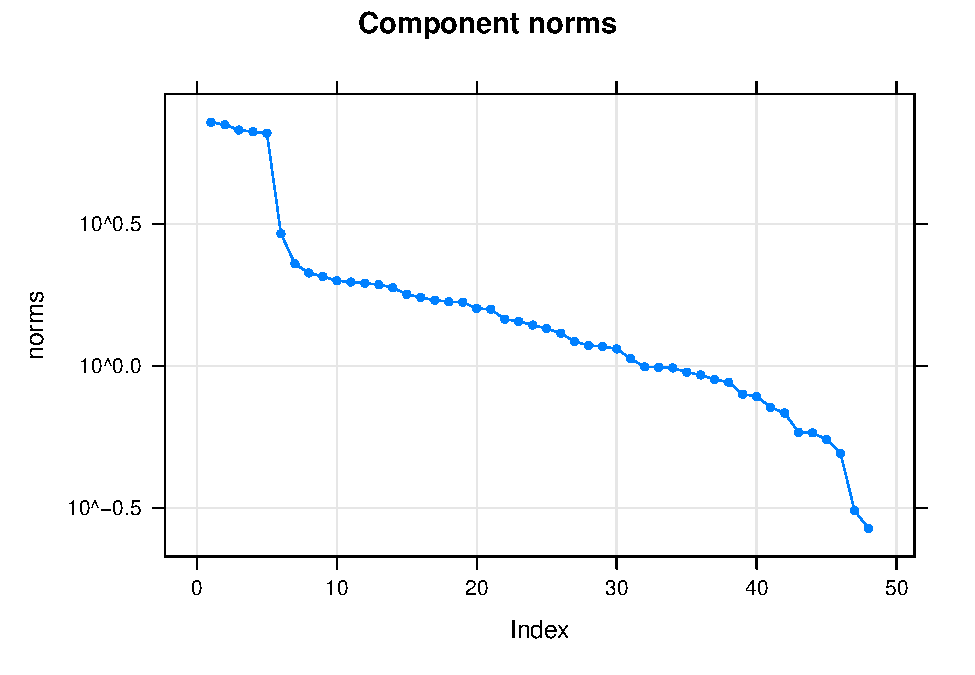
\includegraphics{iossa_example/eigen plot-1.pdf}

\begin{Shaded}
\begin{Highlighting}[]
\NormalTok{  grouping\_num }\OtherTok{\textless{}{-}} \DecValTok{5}
\end{Highlighting}
\end{Shaded}

\hypertarget{ii.-ux430ux432ux442ux43eux43cux430ux442ux438ux447ux435ux441ux43aux43eux435-ux432ux44bux434ux435ux43bux435ux43dux438ux435-ux442ux440ux435ux43dux434ux430}{%
\section{II. Автоматическое выделение
тренда}\label{ii.-ux430ux432ux442ux43eux43cux430ux442ux438ux447ux435ux441ux43aux43eux435-ux432ux44bux434ux435ux43bux435ux43dux438ux435-ux442ux440ux435ux43dux434ux430}}

\begin{Shaded}
\begin{Highlighting}[]
\NormalTok{  g }\OtherTok{\textless{}{-}} \FunctionTok{grouping.auto}\NormalTok{(s, }\AttributeTok{base =} \StringTok{"series"}\NormalTok{, }
                 \AttributeTok{freq.bins =} \FunctionTok{list}\NormalTok{(}\AttributeTok{Tendency =} \DecValTok{1}\SpecialCharTok{/}\DecValTok{240}\NormalTok{, }\AttributeTok{Trend =} \DecValTok{1}\SpecialCharTok{/}\DecValTok{24}\NormalTok{), }
                 \AttributeTok{threshold =} \FloatTok{0.8}\NormalTok{)}
                 
\NormalTok{  trend\_time\_series }\OtherTok{\textless{}{-}} \FunctionTok{reconstruct}\NormalTok{(s, }\AttributeTok{groups =}\NormalTok{ g)}
  
  \FunctionTok{plot}\NormalTok{(trend\_time\_series, }
   \AttributeTok{add.residuals =} \ConstantTok{FALSE}\NormalTok{, }
   \AttributeTok{plot.method =} \StringTok{"xyplot"}\NormalTok{, }\AttributeTok{superpose =} \ConstantTok{TRUE}\NormalTok{)}
\end{Highlighting}
\end{Shaded}

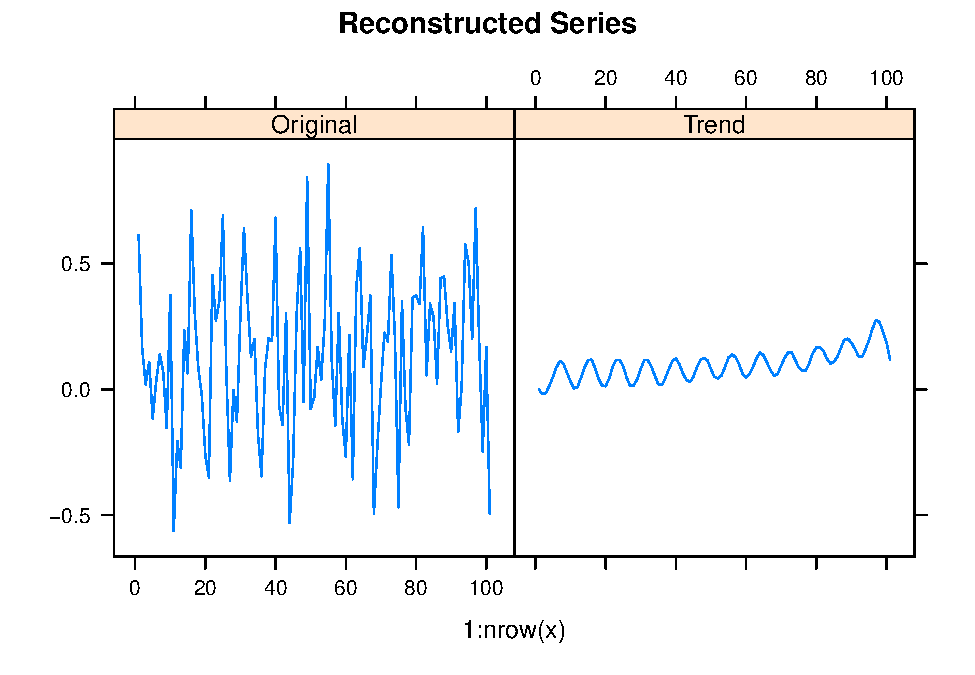
\includegraphics{iossa_example/decomposition-1.pdf}

\hypertarget{iii.-ux432ux44bux434ux435ux43bux435ux43dux438ux435-ux442ux440ux435ux43dux434ux430-ux441-ux43fux43eux43cux43eux449ux44cux44e-iossa}{%
\section{III. Выделение тренда с помощью
iossa}\label{iii.-ux432ux44bux434ux435ux43bux435ux43dux438ux435-ux442ux440ux435ux43dux434ux430-ux441-ux43fux43eux43cux43eux449ux44cux44e-iossa}}

\begin{Shaded}
\begin{Highlighting}[]
\NormalTok{  ioss }\OtherTok{\textless{}{-}} \FunctionTok{iossa}\NormalTok{(s, }\AttributeTok{nested.groups =} \FunctionTok{list}\NormalTok{(}\DecValTok{1}\NormalTok{, }\DecValTok{2}\NormalTok{, }\DecValTok{3}\NormalTok{, }\DecValTok{4}\NormalTok{, }\DecValTok{5}\NormalTok{))}
\NormalTok{  g\_iossa }\OtherTok{\textless{}{-}} \FunctionTok{grouping.auto}\NormalTok{(ioss, }\AttributeTok{base =} \StringTok{"series"}\NormalTok{, }
                 \AttributeTok{freq.bins =} \FunctionTok{list}\NormalTok{(}\AttributeTok{Tendency =} \DecValTok{1}\SpecialCharTok{/}\DecValTok{240}\NormalTok{, }\AttributeTok{Trend =} \DecValTok{1}\SpecialCharTok{/}\DecValTok{24}\NormalTok{), }
                 \AttributeTok{threshold =} \FloatTok{0.8}\NormalTok{)}
                 
\NormalTok{  trend\_time\_series }\OtherTok{\textless{}{-}} \FunctionTok{reconstruct}\NormalTok{(ioss, }\AttributeTok{groups =}\NormalTok{ g\_iossa)}
  
  \FunctionTok{plot}\NormalTok{(trend\_time\_series, }
   \AttributeTok{add.residuals =} \ConstantTok{FALSE}\NormalTok{, }
   \AttributeTok{plot.method =} \StringTok{"xyplot"}\NormalTok{, }\AttributeTok{superpose =} \ConstantTok{TRUE}\NormalTok{)}
\end{Highlighting}
\end{Shaded}

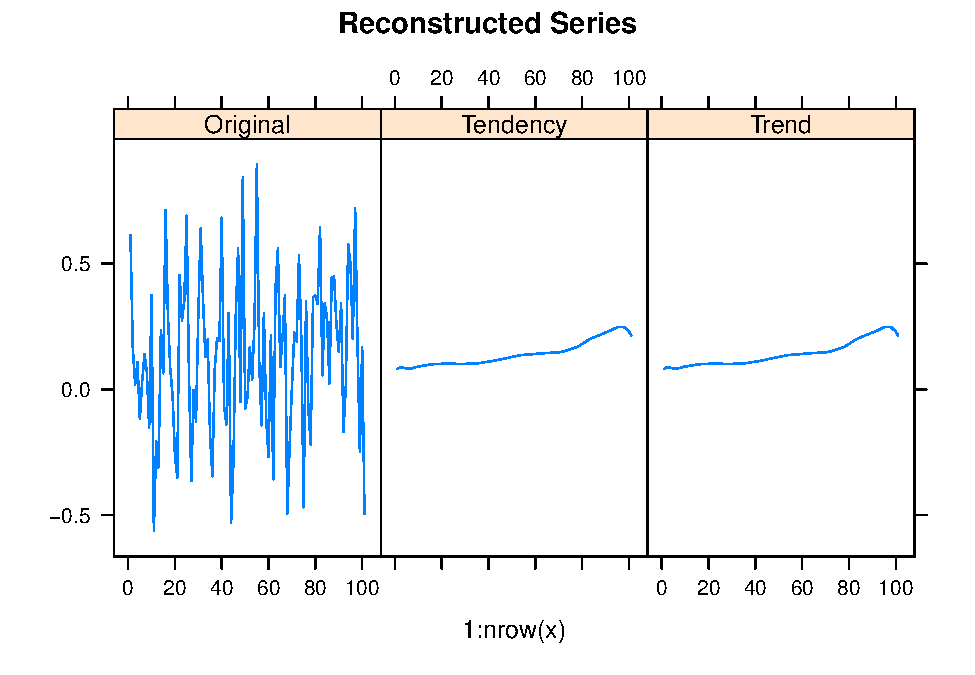
\includegraphics{iossa_example/iossa_trend-1.pdf}

Видно, что автоматическое выделение тренда без решения проблемы
отсутствия сильной разделимости не дало желаемого результата, тренд
смешался с гармоникой. При этом после iossa автоматическое выделение
хорошо сработало, тренд отделился от гармоник. Можно увидеть на графике
тренда экспоненту, как и было задано в начале программы. Из графика норм
собственных чисел следует, что сильной разделимости компонент сигнала
нет, поэтому после iossa можно выполнять автоматическое выделение
тренда.
\section{Эксперимент 2}
\begin{Shaded}
\begin{Highlighting}[]
  \FunctionTok{library}\NormalTok{(}\StringTok{"svd"}\NormalTok{)}
  \FunctionTok{library}\NormalTok{(}\StringTok{"forecast"}\NormalTok{)}
  \FunctionTok{library}\NormalTok{(}\StringTok{"Rssa"}\NormalTok{)}
  \FunctionTok{library}\NormalTok{(}\StringTok{"lattice"}\NormalTok{)}
\end{Highlighting}
\end{Shaded}

\hypertarget{i.-ux441ux43eux437ux434ux430ux43dux438ux435-ux432ux440ux435ux43cux435ux43dux43dux43eux433ux43e-ux440ux44fux434ux430-ux434ux43bux44f-ux43fux440ux438ux43cux435ux43dux435ux43dux438ux44f-ux430ux43bux433ux43eux440ux438ux442ux43cux430}{%
\section{I. Создание временного ряда для применения
алгоритма}\label{i.-ux441ux43eux437ux434ux430ux43dux438ux435-ux432ux440ux435ux43cux435ux43dux43dux43eux433ux43e-ux440ux44fux434ux430-ux434ux43bux44f-ux43fux440ux438ux43cux435ux43dux435ux43dux438ux44f-ux430ux43bux433ux43eux440ux438ux442ux43cux430}}

\begin{Shaded}
\begin{Highlighting}[]
\NormalTok{  trend\_function1 }\OtherTok{\textless{}{-}} \ControlFlowTok{function}\NormalTok{(n)\{}
    \CommentTok{\# Input: аргумент {-} отметка на временной оси}
    \CommentTok{\# Output: значение тренда как функции в точке}
    \FunctionTok{return}\NormalTok{ (}\FloatTok{0.001} \SpecialCharTok{*}\NormalTok{ n }\SpecialCharTok{\^{}} \DecValTok{2} \SpecialCharTok{{-}} \FloatTok{0.5} \SpecialCharTok{*}\NormalTok{ n }\SpecialCharTok{+} \DecValTok{3}\NormalTok{)}
\NormalTok{  \}}
\end{Highlighting}
\end{Shaded}

\begin{Shaded}
\begin{Highlighting}[]
\NormalTok{  harmonic\_component1\_function }\OtherTok{\textless{}{-}} \ControlFlowTok{function}\NormalTok{(n)\{}
    \CommentTok{\# Input: аргумент {-} отметка на временной оси}
    \CommentTok{\# Output: значение гармонической компоненты как функции в точке}
    \FunctionTok{return}\NormalTok{ (}\FloatTok{4.02} \SpecialCharTok{*} \FunctionTok{cos}\NormalTok{(}\DecValTok{2} \SpecialCharTok{*}\NormalTok{ pi }\SpecialCharTok{*}\NormalTok{ n }\SpecialCharTok{/} \DecValTok{3}\NormalTok{))}
\NormalTok{  \}}
\end{Highlighting}
\end{Shaded}

\begin{Shaded}
\begin{Highlighting}[]
  \FunctionTok{set.seed}\NormalTok{(}\DecValTok{11{-}10{-}2021}\NormalTok{)}
\NormalTok{  time\_series }\OtherTok{=} \DecValTok{0}\SpecialCharTok{:}\DecValTok{100}
\NormalTok{  actual\_trend }\OtherTok{\textless{}{-}} \FunctionTok{trend\_function1}\NormalTok{(time\_series)}
\NormalTok{  time\_series }\OtherTok{\textless{}{-}} \FunctionTok{trend\_function1}\NormalTok{(time\_series) }\SpecialCharTok{+}
\\ \FunctionTok{harmonic\_component1\_function}\NormalTok{(time\_series) }\SpecialCharTok{+} \FunctionTok{rnorm}\NormalTok{(}\DecValTok{101}\NormalTok{, }\AttributeTok{sd =} \DecValTok{2}\NormalTok{)}
\end{Highlighting}
\end{Shaded}

Создан временной ряд \(f_n , 0\leqslant n < N, N=101\), с функцией
тренда \(0.001n^2-0.5n+3\) и гармоникой
\(4.02 * \mathsf{cos}(\frac{2\pi n}{3})\), добавлен стандартный гауссовский шум
\(2 \epsilon_n\).

\begin{Shaded}
\begin{Highlighting}[]
\NormalTok{  s }\OtherTok{\textless{}{-}} \FunctionTok{ssa}\NormalTok{(time\_series, }\AttributeTok{L =} \DecValTok{48}\NormalTok{)}
  \FunctionTok{plot}\NormalTok{(s)}
\end{Highlighting}
\end{Shaded}

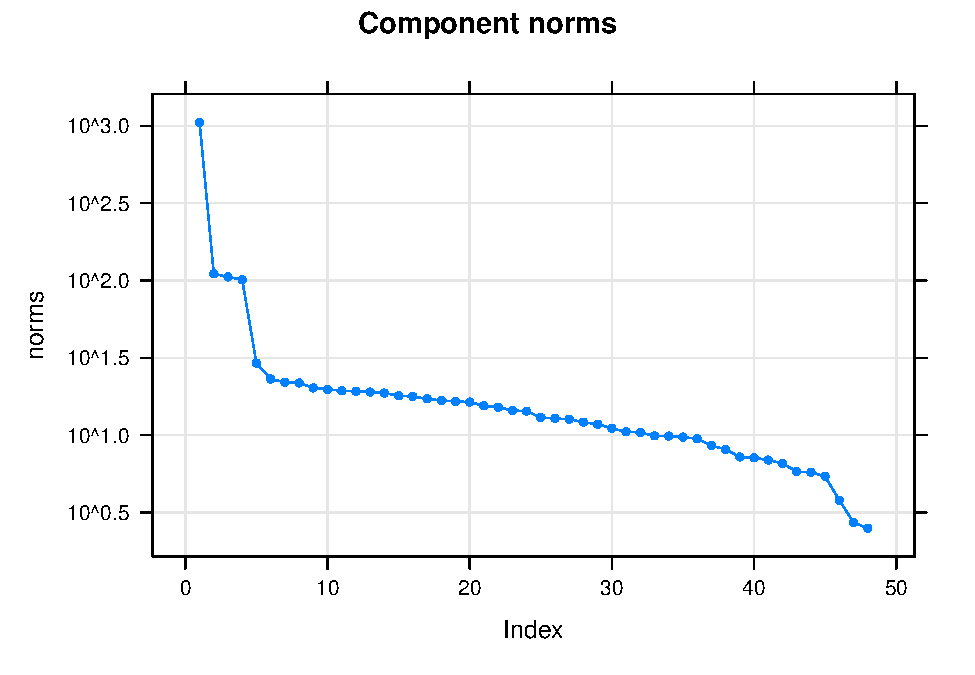
\includegraphics{iossa_example2/eigen plot-1.pdf}

\begin{Shaded}
\begin{Highlighting}[]
  \FunctionTok{plot}\NormalTok{(s, }\AttributeTok{type =} \StringTok{"vectors"}\NormalTok{, }\AttributeTok{idx =} \DecValTok{1}\SpecialCharTok{:}\DecValTok{10}\NormalTok{)}
\end{Highlighting}
\end{Shaded}

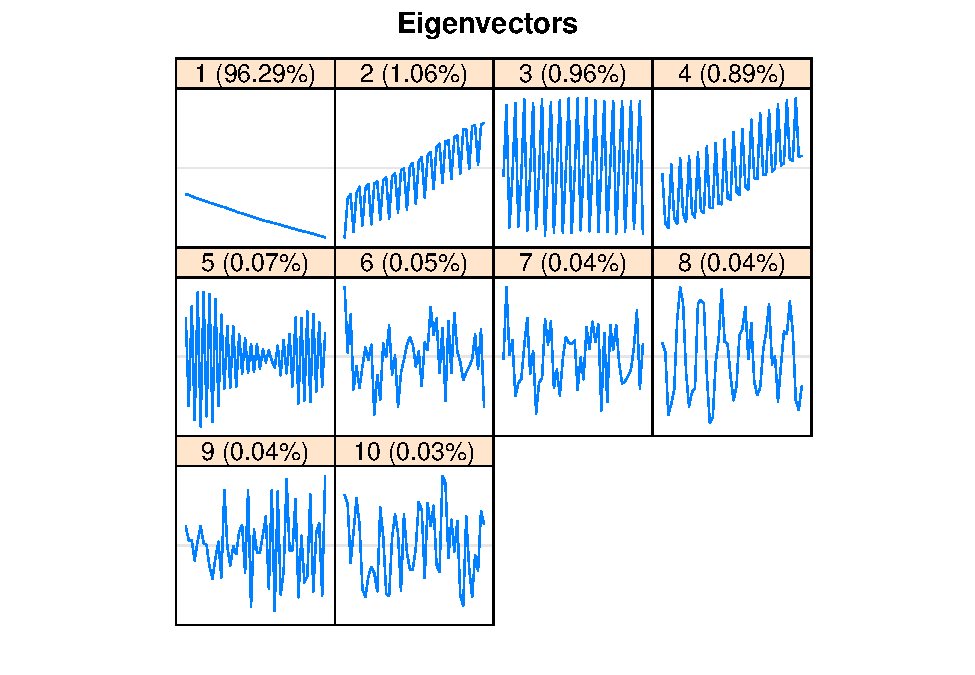
\includegraphics{iossa_example2/vectors_plot-1.pdf}

По графику видно, что сильная разделимость тренда и гармоники
отсутствует.

\hypertarget{ii.-ux430ux432ux442ux43eux43cux430ux442ux438ux447ux435ux441ux43aux43eux435-ux432ux44bux434ux435ux43bux435ux43dux438ux435-ux442ux440ux435ux43dux434ux430}{%
\section{II. Автоматическое выделение
тренда}\label{ii.-ux430ux432ux442ux43eux43cux430ux442ux438ux447ux435ux441ux43aux43eux435-ux432ux44bux434ux435ux43bux435ux43dux438ux435-ux442ux440ux435ux43dux434ux430}}

\begin{Shaded}
\begin{Highlighting}[]
\NormalTok{  g }\OtherTok{\textless{}{-}} \FunctionTok{grouping.auto}\NormalTok{(s, }\AttributeTok{base =} \StringTok{"series"}\NormalTok{, }
                 \AttributeTok{freq.bins =} \FunctionTok{list}\NormalTok{(}\AttributeTok{Tendency =} \DecValTok{1}\SpecialCharTok{/}\DecValTok{240}\NormalTok{, }\AttributeTok{Trend =} \DecValTok{1}\SpecialCharTok{/}\DecValTok{24}\NormalTok{), }
                 \AttributeTok{threshold =} \FloatTok{0.8}\NormalTok{)}
                 
\NormalTok{  trend\_time\_series }\OtherTok{\textless{}{-}} \FunctionTok{reconstruct}\NormalTok{(s, }\AttributeTok{groups =}\NormalTok{ g)}
  
  \FunctionTok{plot}\NormalTok{(trend\_time\_series, }
   \AttributeTok{add.residuals =} \ConstantTok{FALSE}\NormalTok{, }
   \AttributeTok{plot.method =} \StringTok{"xyplot"}\NormalTok{, }\AttributeTok{superpose =} \ConstantTok{TRUE}\NormalTok{)}
\end{Highlighting}
\end{Shaded}

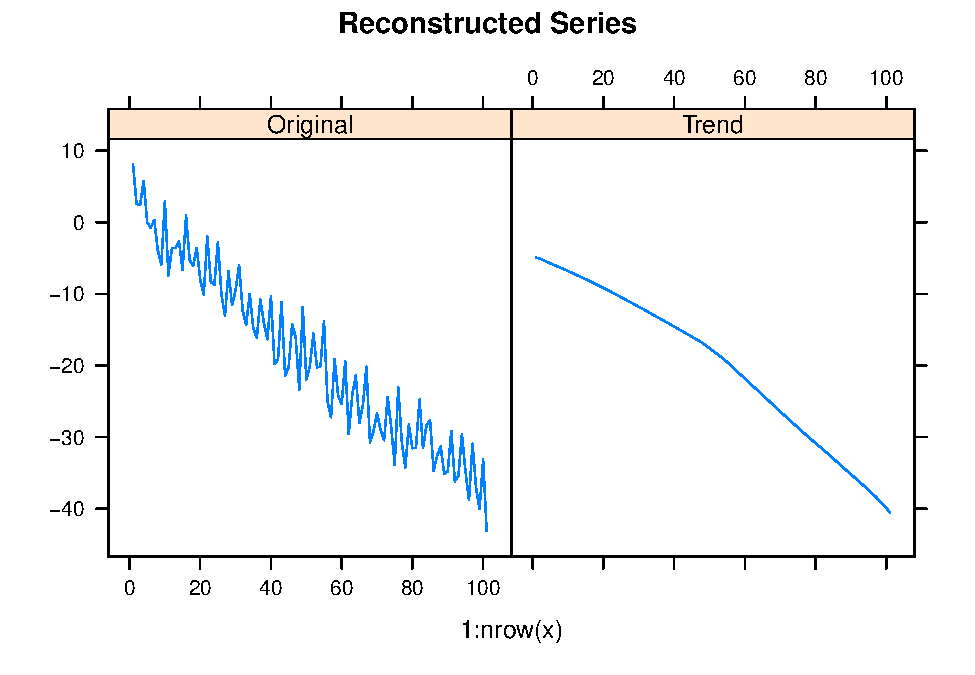
\includegraphics{iossa_example2/decomposition-1.pdf}

\hypertarget{iii.-ux432ux44bux434ux435ux43bux435ux43dux438ux435-ux442ux440ux435ux43dux434ux430-ux441-ux43fux43eux43cux43eux449ux44cux44e-iossa}{%
\section{III. Выделение тренда с помощью
iossa}\label{iii.-ux432ux44bux434ux435ux43bux435ux43dux438ux435-ux442ux440ux435ux43dux434ux430-ux441-ux43fux43eux43cux43eux449ux44cux44e-iossa}}

\begin{Shaded}
\begin{Highlighting}[]
\NormalTok{  ioss }\OtherTok{\textless{}{-}} \FunctionTok{iossa}\NormalTok{(s, }\AttributeTok{nested.groups =} \FunctionTok{list}\NormalTok{(}\DecValTok{1}\NormalTok{, }\DecValTok{2}\NormalTok{, }\DecValTok{3}\NormalTok{, }\DecValTok{4}\NormalTok{, }\DecValTok{5}\NormalTok{))}
\NormalTok{  g\_iossa }\OtherTok{\textless{}{-}} \FunctionTok{grouping.auto}\NormalTok{(ioss, }\AttributeTok{base =} \StringTok{"series"}\NormalTok{, }
                 \AttributeTok{freq.bins =} \FunctionTok{list}\NormalTok{(}\AttributeTok{Tendency =} \DecValTok{1}\SpecialCharTok{/}\DecValTok{240}\NormalTok{, }\AttributeTok{Trend =} \DecValTok{1}\SpecialCharTok{/}\DecValTok{24}\NormalTok{), }
                 \AttributeTok{threshold =} \FloatTok{0.8}\NormalTok{)}
                 
\NormalTok{  trend\_time\_series\_iossa }\OtherTok{\textless{}{-}} \FunctionTok{reconstruct}\NormalTok{(ioss, }\AttributeTok{groups =}\NormalTok{ g\_iossa)}
  
  \FunctionTok{plot}\NormalTok{(trend\_time\_series\_iossa, }
   \AttributeTok{add.residuals =} \ConstantTok{FALSE}\NormalTok{, }
   \AttributeTok{plot.method =} \StringTok{"xyplot"}\NormalTok{, }\AttributeTok{superpose =} \ConstantTok{TRUE}\NormalTok{)}
\end{Highlighting}
\end{Shaded}

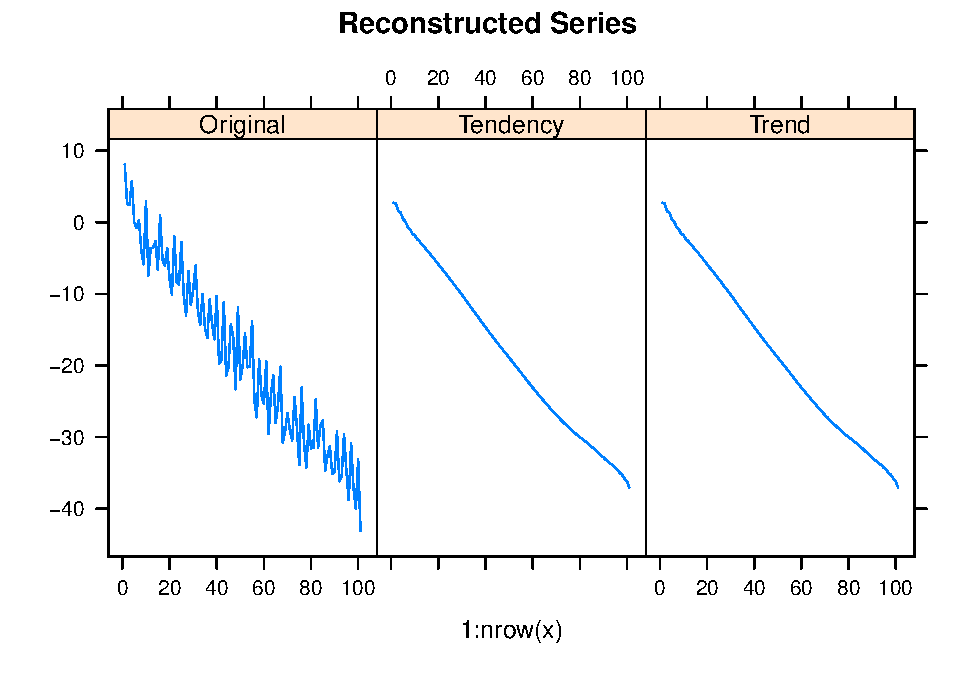
\includegraphics{iossa_example2/iossa_trend-1.pdf}

\hypertarget{iv.-ux441ux440ux430ux432ux43dux435ux43dux438ux435-ux440ux435ux437ux443ux43bux44cux442ux430ux442ux43eux432}{%
\section{IV. Сравнение
результатов}\label{iv.-ux441ux440ux430ux432ux43dux435ux43dux438ux435-ux440ux435ux437ux443ux43bux44cux442ux430ux442ux43eux432}}

\begin{Shaded}
\begin{Highlighting}[]
  \FunctionTok{library}\NormalTok{(ggplot2)}
  \FunctionTok{library}\NormalTok{(dplyr)}
  \FunctionTok{library}\NormalTok{(tidyr)}
  
\NormalTok{  x }\OtherTok{\textless{}{-}} \DecValTok{0}\SpecialCharTok{:}\DecValTok{100}
\NormalTok{  iossa\_auto\_trend }\OtherTok{\textless{}{-}}\NormalTok{ trend\_time\_series\_iossa}\SpecialCharTok{\$}\NormalTok{Trend}
\NormalTok{  auto\_trend }\OtherTok{\textless{}{-}}\NormalTok{ trend\_time\_series}\SpecialCharTok{\$}\NormalTok{Trend}
\NormalTok{  plot\_df }\OtherTok{\textless{}{-}} \FunctionTok{tbl\_df}\NormalTok{(}\FunctionTok{data.frame}\NormalTok{(x, iossa\_auto\_trend, auto\_trend, actual\_trend))}
\NormalTok{  plot\_df }\SpecialCharTok{\%\textgreater{}\%} \FunctionTok{gather}\NormalTok{(}\StringTok{"Trend"}\NormalTok{, }\StringTok{"Value"}\NormalTok{, }\SpecialCharTok{{-}}\NormalTok{x) }\SpecialCharTok{\%\textgreater{}\%} \FunctionTok{ggplot}\NormalTok{(}\FunctionTok{aes}\NormalTok{(x, Value)) }\SpecialCharTok{+} 
\\ \FunctionTok{geom\_line}\NormalTok{(}\FunctionTok{aes}\NormalTok{(}\AttributeTok{color =}\NormalTok{ Trend), }\AttributeTok{size =} \DecValTok{1}\NormalTok{)}
\end{Highlighting}
\end{Shaded}

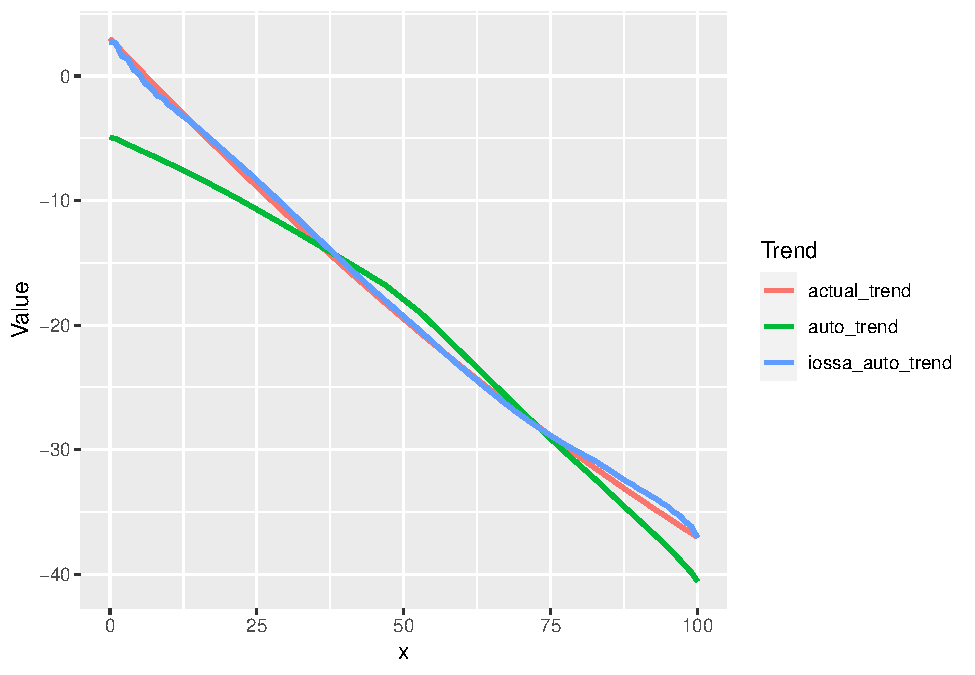
\includegraphics{iossa_example2/comparing-1.pdf}

Как можно увидеть, автоматическое выделение тренда без применения iossa
привело к смешиванию тренда и гармоники: кривая полученного тренда
сильно отклоняется от фактического тренда, в то же время с применением
iossa тренд выделился правильно.

\section{Эксперимент 3}
\begin{Shaded}
\begin{Highlighting}[]
  \FunctionTok{library}\NormalTok{(}\StringTok{"svd"}\NormalTok{)}
  \FunctionTok{library}\NormalTok{(}\StringTok{"forecast"}\NormalTok{)}
  \FunctionTok{library}\NormalTok{(}\StringTok{"Rssa"}\NormalTok{)}
  \FunctionTok{library}\NormalTok{(}\StringTok{"lattice"}\NormalTok{)}
  \FunctionTok{library}\NormalTok{(}\StringTok{"parallel"}\NormalTok{)}
  \FunctionTok{library}\NormalTok{(}\StringTok{"doParallel"}\NormalTok{)}
  \FunctionTok{library}\NormalTok{(}\StringTok{"doRNG"}\NormalTok{)}
\end{Highlighting}
\end{Shaded}

\begin{Shaded}
\begin{Highlighting}[]
\NormalTok{    trend\_function1 }\OtherTok{\textless{}{-}} \ControlFlowTok{function}\NormalTok{(n)\{}
      \CommentTok{\# Input: аргумент {-} отметка на временной оси}
      \CommentTok{\# Output: значение тренда как функции в точке}
      \FunctionTok{return}\NormalTok{ (}\FloatTok{0.001} \SpecialCharTok{*}\NormalTok{ n }\SpecialCharTok{\^{}} \DecValTok{2} \SpecialCharTok{{-}} \FloatTok{0.5} \SpecialCharTok{*}\NormalTok{ n }\SpecialCharTok{+} \DecValTok{3}\NormalTok{)}
\NormalTok{    \}}
\end{Highlighting}
\end{Shaded}

\begin{Shaded}
\begin{Highlighting}[]
\NormalTok{  harmonic\_component1\_function }\OtherTok{\textless{}{-}} \ControlFlowTok{function}\NormalTok{(n)\{}
    \CommentTok{\# Input: аргумент {-} отметка на временной оси}
    \CommentTok{\# Output: значение гармонической компоненты как функции в точке}
    \FunctionTok{return}\NormalTok{ (}\FloatTok{4.02} \SpecialCharTok{*} \FunctionTok{cos}\NormalTok{(}\DecValTok{2} \SpecialCharTok{*}\NormalTok{ pi }\SpecialCharTok{*}\NormalTok{ n }\SpecialCharTok{/} \DecValTok{3}\NormalTok{))}
\NormalTok{  \}}
\end{Highlighting}
\end{Shaded}

\begin{Shaded}
\begin{Highlighting}[]
  \FunctionTok{set.seed}\NormalTok{(}\DecValTok{11{-}10{-}2021}\NormalTok{)}
\NormalTok{  time\_series\_stamps }\OtherTok{=} \DecValTok{0}\SpecialCharTok{:}\DecValTok{100}
\NormalTok{  actual\_trend }\OtherTok{\textless{}{-}} \FunctionTok{trend\_function1}\NormalTok{(time\_series\_stamps)}
\NormalTok{  refined\_time\_series }\OtherTok{\textless{}{-}}\NormalTok{ actual\_trend }\SpecialCharTok{+} \FunctionTok{harmonic\_component1\_function}\NormalTok{(time\_series\_stamps)}
\end{Highlighting}
\end{Shaded}

\begin{Shaded}
\begin{Highlighting}[]
  \FunctionTok{print}\NormalTok{(}\FunctionTok{Sys.time}\NormalTok{())}
\end{Highlighting}
\end{Shaded}

\begin{verbatim}
## [1] "2022-06-04 14:03:18 MSK"
\end{verbatim}

\begin{Shaded}
\begin{Highlighting}[]
\NormalTok{  cores }\OtherTok{\textless{}{-}} \FunctionTok{detectCores}\NormalTok{()}
\NormalTok{  cl }\OtherTok{\textless{}{-}} \FunctionTok{makeCluster}\NormalTok{(cores[}\DecValTok{1}\NormalTok{] }\SpecialCharTok{{-}} \DecValTok{1}\NormalTok{)}
  \FunctionTok{registerDoParallel}\NormalTok{(cl)}
\NormalTok{  M }\OtherTok{\textless{}{-}} \DecValTok{100}
  
\NormalTok{  st }\OtherTok{\textless{}{-}} \FunctionTok{system.time}\NormalTok{(rejectEV }\OtherTok{\textless{}{-}} \FunctionTok{foreach}\NormalTok{(}
    \AttributeTok{i =} \DecValTok{1}\SpecialCharTok{:}\NormalTok{M,}
    \AttributeTok{.export =} \FunctionTok{c}\NormalTok{(}\StringTok{\textquotesingle{}ssa\textquotesingle{}}\NormalTok{, }\StringTok{\textquotesingle{}rnorm\textquotesingle{}}\NormalTok{, }\StringTok{\textquotesingle{}reconstruct\textquotesingle{}}\NormalTok{, }\StringTok{\textquotesingle{}iossa\textquotesingle{}}\NormalTok{, }\StringTok{\textquotesingle{}mean\textquotesingle{}}\NormalTok{, }\StringTok{\textquotesingle{}sort\textquotesingle{}}\NormalTok{, }\StringTok{\textquotesingle{}grouping.auto\textquotesingle{}}\NormalTok{),}
    \AttributeTok{.combine =}\NormalTok{ rbind}
\NormalTok{  ) }\SpecialCharTok{\%dorng\%}\NormalTok{ \{}
\NormalTok{    time\_series }\OtherTok{\textless{}{-}}\NormalTok{ refined\_time\_series }\SpecialCharTok{+} \FunctionTok{rnorm}\NormalTok{(}\DecValTok{101}\NormalTok{, }\AttributeTok{mean =} \DecValTok{0}\NormalTok{, }\AttributeTok{sd =} \DecValTok{2}\NormalTok{)}
    
\NormalTok{    s }\OtherTok{\textless{}{-}} \FunctionTok{ssa}\NormalTok{(time\_series, }\AttributeTok{L =} \DecValTok{48}\NormalTok{)}
\NormalTok{    grouping\_num }\OtherTok{\textless{}{-}} \DecValTok{5}
    
    \CommentTok{\#iossa with 5 separate groups}
\NormalTok{    ioss5 }\OtherTok{\textless{}{-}} \FunctionTok{iossa}\NormalTok{(s, }\AttributeTok{nested.groups =} \FunctionTok{list}\NormalTok{(}\DecValTok{1}\NormalTok{, }\DecValTok{2}\NormalTok{, }\DecValTok{3}\NormalTok{, }\DecValTok{4}\NormalTok{, }\DecValTok{5}\NormalTok{))}
\NormalTok{    g\_iossa5 }\OtherTok{\textless{}{-}} \FunctionTok{grouping.auto}\NormalTok{(ioss5, }\AttributeTok{base =} \StringTok{"series"}\NormalTok{, }
                   \AttributeTok{freq.bins =} \FunctionTok{list}\NormalTok{(}\AttributeTok{Tendency =} \DecValTok{1}\SpecialCharTok{/}\DecValTok{240}\NormalTok{, }\AttributeTok{Trend =} \DecValTok{1}\SpecialCharTok{/}\DecValTok{24}\NormalTok{), }
                   \AttributeTok{threshold =} \FloatTok{0.8}\NormalTok{)}
                   
\NormalTok{    trend\_time\_series\_iossa5 }\OtherTok{\textless{}{-}} \FunctionTok{reconstruct}\NormalTok{(ioss5, }\AttributeTok{groups =}\NormalTok{ g\_iossa5)}\SpecialCharTok{\$}\NormalTok{Trend}
    
    \CommentTok{\#iossa with 2 groups}
\NormalTok{    ioss2 }\OtherTok{\textless{}{-}} \FunctionTok{iossa}\NormalTok{(s, }\AttributeTok{nested.groups =} \FunctionTok{list}\NormalTok{(}\FunctionTok{c}\NormalTok{(}\DecValTok{1}\NormalTok{, }\DecValTok{2}\NormalTok{, }\DecValTok{4}\NormalTok{), }\FunctionTok{c}\NormalTok{(}\DecValTok{3}\NormalTok{, }\DecValTok{5}\NormalTok{)))}
\NormalTok{    g\_iossa2 }\OtherTok{\textless{}{-}} \FunctionTok{grouping.auto}\NormalTok{(ioss2, }\AttributeTok{base =} \StringTok{"series"}\NormalTok{, }
                   \AttributeTok{freq.bins =} \FunctionTok{list}\NormalTok{(}\AttributeTok{Tendency =} \DecValTok{1}\SpecialCharTok{/}\DecValTok{240}\NormalTok{, }\AttributeTok{Trend =} \DecValTok{1}\SpecialCharTok{/}\DecValTok{24}\NormalTok{), }
                   \AttributeTok{threshold =} \FloatTok{0.8}\NormalTok{)}
                   
\NormalTok{    trend\_time\_series\_iossa2 }\OtherTok{\textless{}{-}} \FunctionTok{reconstruct}\NormalTok{(ioss2, }\AttributeTok{groups =}\NormalTok{ g\_iossa2)}\SpecialCharTok{\$}\NormalTok{Trend}
    
    \FunctionTok{data.frame}\NormalTok{(}\AttributeTok{mse\_5\_groups =} \FunctionTok{mean}\NormalTok{((trend\_time\_series\_iossa5 }\SpecialCharTok{{-}}\NormalTok{ actual\_trend) }\SpecialCharTok{\^{}} \DecValTok{2}\NormalTok{), }
               \AttributeTok{mse\_2\_groups =} \FunctionTok{mean}\NormalTok{((trend\_time\_series\_iossa2 }\SpecialCharTok{{-}}\NormalTok{ actual\_trend) }\SpecialCharTok{\^{}} \DecValTok{2}\NormalTok{))}
\NormalTok{  \})}
  
  \FunctionTok{stopCluster}\NormalTok{(cl)}
  \CommentTok{\#print(rejectEV)}
  \CommentTok{\#Средняя MSE для iossa с 5{-}ю группами:}
  \FunctionTok{print}\NormalTok{(}\FunctionTok{mean}\NormalTok{(rejectEV[[}\DecValTok{1}\NormalTok{]]))}
\end{Highlighting}
\end{Shaded}

\begin{verbatim}
## [1] 0.2287474
\end{verbatim}

\begin{Shaded}
\begin{Highlighting}[]
  \CommentTok{\#Средняя MSE для iossa с 2{-}мя группами:}
  \FunctionTok{print}\NormalTok{(}\FunctionTok{mean}\NormalTok{(rejectEV[[}\DecValTok{2}\NormalTok{]]))}
\end{Highlighting}
\end{Shaded}

\begin{verbatim}
## [1] 0.2233865
\end{verbatim}

\section{Эксперимент 4}

\begin{Shaded}
\begin{Highlighting}[]
  \FunctionTok{library}\NormalTok{(}\StringTok{"svd"}\NormalTok{)}
  \FunctionTok{library}\NormalTok{(}\StringTok{"forecast"}\NormalTok{)}
  \FunctionTok{library}\NormalTok{(}\StringTok{"Rssa"}\NormalTok{)}
  \FunctionTok{library}\NormalTok{(}\StringTok{"lattice"}\NormalTok{)}
  \FunctionTok{library}\NormalTok{(}\StringTok{"parallel"}\NormalTok{)}
  \FunctionTok{library}\NormalTok{(}\StringTok{"doParallel"}\NormalTok{)}
  \FunctionTok{library}\NormalTok{(}\StringTok{"doRNG"}\NormalTok{)}
\end{Highlighting}
\end{Shaded}

\begin{Shaded}
\begin{Highlighting}[]
\NormalTok{    trend\_function1 }\OtherTok{\textless{}{-}} \ControlFlowTok{function}\NormalTok{(n)\{}
      \CommentTok{\# Input: аргумент {-} отметка на временной оси}
      \CommentTok{\# Output: значение тренда как функции в точке}
      \FunctionTok{return}\NormalTok{ (}\DecValTok{2} \SpecialCharTok{*} \FunctionTok{exp}\NormalTok{(}\FloatTok{0.03} \SpecialCharTok{*}\NormalTok{ n) }\SpecialCharTok{{-}} \FloatTok{0.1} \SpecialCharTok{*}\NormalTok{ n }\SpecialCharTok{{-}} \DecValTok{20}\NormalTok{)}
\NormalTok{    \}}
\end{Highlighting}
\end{Shaded}

\begin{Shaded}
\begin{Highlighting}[]
\NormalTok{    harmonic\_component1\_function }\OtherTok{\textless{}{-}} \ControlFlowTok{function}\NormalTok{(n)\{}
      \CommentTok{\# Input: аргумент {-} отметка на временной оси}
      \CommentTok{\# Output: значение гармонической компоненты как функции в точке}
      \FunctionTok{return}\NormalTok{ (}\FloatTok{5.2} \SpecialCharTok{*} \FunctionTok{cos}\NormalTok{(}\DecValTok{2} \SpecialCharTok{*}\NormalTok{ pi }\SpecialCharTok{*}\NormalTok{ n }\SpecialCharTok{/} \DecValTok{6} \SpecialCharTok{+}\NormalTok{ pi }\SpecialCharTok{/} \DecValTok{4}\NormalTok{))}
\NormalTok{    \}}
\end{Highlighting}
\end{Shaded}

\begin{Shaded}
\begin{Highlighting}[]
\NormalTok{    harmonic\_component2\_function }\OtherTok{\textless{}{-}} \ControlFlowTok{function}\NormalTok{(n)\{}
      \CommentTok{\# Input: аргумент {-} отметка на временной оси}
      \CommentTok{\# Output: значение гармонической компоненты как функции в точке}
      \FunctionTok{return}\NormalTok{ (}\FloatTok{5.2} \SpecialCharTok{*} \FunctionTok{cos}\NormalTok{(}\DecValTok{2} \SpecialCharTok{*}\NormalTok{ pi }\SpecialCharTok{*}\NormalTok{ n }\SpecialCharTok{/} \DecValTok{3}\NormalTok{))}
\NormalTok{    \}}
\end{Highlighting}
\end{Shaded}

\begin{Shaded}
\begin{Highlighting}[]
    \FunctionTok{set.seed}\NormalTok{(}\DecValTok{11{-}10{-}2021}\NormalTok{)}
\NormalTok{    time\_series\_stamps }\OtherTok{=} \DecValTok{0}\SpecialCharTok{:}\DecValTok{100}
\NormalTok{    actual\_trend }\OtherTok{\textless{}{-}} \FunctionTok{trend\_function1}\NormalTok{(time\_series\_stamps)}
\NormalTok{    refined\_time\_series }\OtherTok{\textless{}{-}}\NormalTok{ actual\_trend }\SpecialCharTok{+}
\\ \FunctionTok{harmonic\_component1\_function}\NormalTok{(time\_series\_stamps) }\SpecialCharTok{+}
\\ \FunctionTok{harmonic\_component2\_function}\NormalTok{(time\_series\_stamps)}
\NormalTok{    harmonics }\OtherTok{\textless{}{-}}\NormalTok{ refined\_time\_series }\SpecialCharTok{{-}}\NormalTok{ actual\_trend}
\end{Highlighting}
\end{Shaded}

\begin{Shaded}
\begin{Highlighting}[]
  \CommentTok{\#tol = 1e{-}3, maxiter = 1000, 1000 launches}

  \FunctionTok{print}\NormalTok{(}\FunctionTok{Sys.time}\NormalTok{())}
\end{Highlighting}
\end{Shaded}

\begin{verbatim}
## [1] "2022-06-04 14:14:56 MSK"
\end{verbatim}

\begin{Shaded}
\begin{Highlighting}[]
\NormalTok{  cores }\OtherTok{\textless{}{-}} \FunctionTok{detectCores}\NormalTok{()}
\NormalTok{  cl }\OtherTok{\textless{}{-}} \FunctionTok{makeCluster}\NormalTok{(cores[}\DecValTok{1}\NormalTok{] }\SpecialCharTok{{-}} \DecValTok{1}\NormalTok{)}
  \FunctionTok{registerDoParallel}\NormalTok{(cl)}
\NormalTok{  M }\OtherTok{\textless{}{-}} \DecValTok{100}
\NormalTok{  signal\_comp\_num }\OtherTok{\textless{}{-}} \DecValTok{6}
  
\NormalTok{  st }\OtherTok{\textless{}{-}} \FunctionTok{system.time}\NormalTok{(rejectEV }\OtherTok{\textless{}{-}} \FunctionTok{foreach}\NormalTok{(}
    \AttributeTok{i =} \DecValTok{1}\SpecialCharTok{:}\NormalTok{M,}
    \AttributeTok{.export =} \FunctionTok{c}\NormalTok{(}\StringTok{\textquotesingle{}ssa\textquotesingle{}}\NormalTok{, }\StringTok{\textquotesingle{}rnorm\textquotesingle{}}\NormalTok{, }\StringTok{\textquotesingle{}reconstruct\textquotesingle{}}\NormalTok{, }\StringTok{\textquotesingle{}iossa\textquotesingle{}}\NormalTok{, }\StringTok{\textquotesingle{}mean\textquotesingle{}}\NormalTok{, }\StringTok{\textquotesingle{}sort\textquotesingle{}}\NormalTok{, }
    \\ \StringTok{\textquotesingle{}grouping.auto\textquotesingle{}}\NormalTok{, }\StringTok{\textquotesingle{}attr\textquotesingle{}}\NormalTok{),}
    \AttributeTok{.combine =}\NormalTok{ rbind}
\NormalTok{  ) }\SpecialCharTok{\%dorng\%}\NormalTok{ \{}
    
\NormalTok{    time\_series }\OtherTok{\textless{}{-}}\NormalTok{ refined\_time\_series }\SpecialCharTok{+} \FunctionTok{rnorm}\NormalTok{(}\DecValTok{101}\NormalTok{, }\AttributeTok{mean =} \DecValTok{0}\NormalTok{, }\AttributeTok{sd =} \FloatTok{0.2}\NormalTok{)}
\NormalTok{    res }\OtherTok{\textless{}{-}}\NormalTok{ refined\_time\_series }\SpecialCharTok{{-}}\NormalTok{ actual\_trend}
    
\NormalTok{    s }\OtherTok{\textless{}{-}} \FunctionTok{ssa}\NormalTok{(time\_series, }\AttributeTok{L =} \DecValTok{48}\NormalTok{)}
    
    \CommentTok{\#iossa with 2 groups (auto grouping)}
\NormalTok{    auto\_grouping }\OtherTok{\textless{}{-}} \FunctionTok{grouping.auto}\NormalTok{(s, }\AttributeTok{base =} \StringTok{"series"}\NormalTok{, }
                    \AttributeTok{freq.bins =} \FunctionTok{list}\NormalTok{(}\AttributeTok{Tendency =} \DecValTok{1}\SpecialCharTok{/}\DecValTok{240}\NormalTok{, }\AttributeTok{Trend =} \DecValTok{1}\SpecialCharTok{/}\DecValTok{24}\NormalTok{), }
                    \AttributeTok{threshold =} \FloatTok{0.7}\NormalTok{)}
    
\NormalTok{    trend\_comp\_all }\OtherTok{\textless{}{-}}\NormalTok{ auto\_grouping}\SpecialCharTok{\$}\NormalTok{Trend}
\NormalTok{    trend\_comp\_signal }\OtherTok{\textless{}{-}}\NormalTok{ trend\_comp\_all[trend\_comp\_all }\SpecialCharTok{\%in\%} \DecValTok{1}\SpecialCharTok{:}\NormalTok{signal\_comp\_num]}
\NormalTok{    signal\_indices }\OtherTok{\textless{}{-}} \DecValTok{1}\SpecialCharTok{:}\NormalTok{signal\_comp\_num}
\NormalTok{    res\_comp }\OtherTok{\textless{}{-}}\NormalTok{ signal\_indices[}\SpecialCharTok{!}\NormalTok{signal\_indices }\SpecialCharTok{\%in\%}\NormalTok{ trend\_comp\_signal]}
    
\NormalTok{    ioss2\_auto }\OtherTok{\textless{}{-}} \FunctionTok{iossa}\NormalTok{(s, }\AttributeTok{nested.groups =} \FunctionTok{list}\NormalTok{(trend\_comp\_signal, res\_comp), }\AttributeTok{tol =} \FloatTok{1e{-}3}\NormalTok{, }
\\ \AttributeTok{maxiter =} \DecValTok{1000}\NormalTok{)}
\NormalTok{    rec2\_auto }\OtherTok{\textless{}{-}} \FunctionTok{reconstruct}\NormalTok{(ioss2\_auto, }\AttributeTok{groups =}\NormalTok{ ioss2\_auto}\SpecialCharTok{\$}\NormalTok{iossa.groups)}
    
\NormalTok{    trend\_time\_series\_iossa2\_auto }\OtherTok{\textless{}{-}}\NormalTok{ rec2\_auto}\SpecialCharTok{\$}\NormalTok{F1}
\NormalTok{    residuals\_time\_series2\_auto }\OtherTok{\textless{}{-}}\NormalTok{ rec2\_auto}\SpecialCharTok{\$}\NormalTok{F2}
    
    \CommentTok{\#iossa with 6 separate groups (no grouping)}
\NormalTok{    ioss5 }\OtherTok{\textless{}{-}} \FunctionTok{iossa}\NormalTok{(s, }\AttributeTok{nested.groups =} \FunctionTok{list}\NormalTok{(}\DecValTok{1}\NormalTok{, }\DecValTok{2}\NormalTok{, }\DecValTok{3}\NormalTok{, }\DecValTok{4}\NormalTok{, }\DecValTok{5}\NormalTok{, }\DecValTok{6}\NormalTok{), }\AttributeTok{tol =} \FloatTok{1e{-}3}\NormalTok{, }\AttributeTok{maxiter =} \DecValTok{1000}\NormalTok{)}
\NormalTok{    g0\_iossa5 }\OtherTok{\textless{}{-}} \FunctionTok{grouping.auto}\NormalTok{(ioss5, }\AttributeTok{base =} \StringTok{"series"}\NormalTok{, }
                    \AttributeTok{freq.bins =} \FunctionTok{list}\NormalTok{(}\AttributeTok{Tendency =} \DecValTok{1}\SpecialCharTok{/}\DecValTok{240}\NormalTok{, }\AttributeTok{Trend =} \DecValTok{1}\SpecialCharTok{/}\DecValTok{24}\NormalTok{), }
                    \AttributeTok{threshold =} \FloatTok{0.7}\NormalTok{)}
                   
\NormalTok{    rec5 }\OtherTok{\textless{}{-}} \FunctionTok{reconstruct}\NormalTok{(ioss5, }\AttributeTok{groups =}\NormalTok{ g0\_iossa5)}
\NormalTok{    trend\_time\_series\_iossa5 }\OtherTok{\textless{}{-}}\NormalTok{ rec5}\SpecialCharTok{\$}\NormalTok{Trend}
\NormalTok{    residuals\_time\_series5 }\OtherTok{\textless{}{-}} \FunctionTok{attr}\NormalTok{(rec5, }\StringTok{"residuals"}\NormalTok{) }\SpecialCharTok{{-}}
\\ \FunctionTok{attr}\NormalTok{(}\FunctionTok{reconstruct}\NormalTok{(ioss5, }\AttributeTok{groups =}\NormalTok{ ioss5}\SpecialCharTok{\$}\NormalTok{iossa.groups), }\StringTok{"residuals"}\NormalTok{)}
    
    \CommentTok{\#iossa with 2 groups (manual grouping)}
\NormalTok{    ioss2 }\OtherTok{\textless{}{-}} \FunctionTok{iossa}\NormalTok{(s, }\AttributeTok{nested.groups =} \FunctionTok{list}\NormalTok{(}\DecValTok{1}\SpecialCharTok{:}\DecValTok{2}\NormalTok{, }\DecValTok{3}\SpecialCharTok{:}\DecValTok{6}\NormalTok{), }\AttributeTok{tol =} \FloatTok{1e{-}3}\NormalTok{, }\AttributeTok{maxiter =} \DecValTok{1000}\NormalTok{)}
\NormalTok{    rec2 }\OtherTok{\textless{}{-}} \FunctionTok{reconstruct}\NormalTok{(ioss2, }\AttributeTok{groups =}\NormalTok{ ioss2}\SpecialCharTok{\$}\NormalTok{iossa.groups)}
    
\NormalTok{    trend\_time\_series\_iossa2 }\OtherTok{\textless{}{-}}\NormalTok{ rec2}\SpecialCharTok{\$}\NormalTok{F1}
\NormalTok{    residuals\_time\_series2 }\OtherTok{\textless{}{-}}\NormalTok{ rec2}\SpecialCharTok{\$}\NormalTok{F2}
    
    \FunctionTok{data.frame}\NormalTok{(}\AttributeTok{mse\_no\_grouping\_trend =} 
    \\ \FunctionTok{mean}\NormalTok{((trend\_time\_series\_iossa5 }\SpecialCharTok{{-}}\NormalTok{ actual\_trend) }\SpecialCharTok{\^{}} \DecValTok{2}\NormalTok{),}
               \AttributeTok{mse\_no\_grouping\_residuals =}
               \\ \FunctionTok{mean}\NormalTok{((residuals\_time\_series5 }\SpecialCharTok{{-}}\NormalTok{ res) }\SpecialCharTok{\^{}} \DecValTok{2}\NormalTok{),}
               \AttributeTok{iter\_no\_grouping =}\NormalTok{ ioss5}\SpecialCharTok{\$}\NormalTok{iossa.result}\SpecialCharTok{\$}\NormalTok{iter,}
               \AttributeTok{mse\_2\_groups\_manual\_trend =}
               \\ \FunctionTok{mean}\NormalTok{((trend\_time\_series\_iossa2 }\SpecialCharTok{{-}}\NormalTok{ actual\_trend) }\SpecialCharTok{\^{}} \DecValTok{2}\NormalTok{),}
               \AttributeTok{mse\_2\_groups\_manual\_residuals =}
               \\ \FunctionTok{mean}\NormalTok{((residuals\_time\_series2 }\SpecialCharTok{{-}}\NormalTok{ res) }\SpecialCharTok{\^{}} \DecValTok{2}\NormalTok{),}
               \AttributeTok{iter\_2\_groups\_manual =}\NormalTok{ ioss2}\SpecialCharTok{\$}\NormalTok{iossa.result}\SpecialCharTok{\$}\NormalTok{iter,}
               \AttributeTok{mse\_auto\_grouping\_trend =}
               \\ \FunctionTok{mean}\NormalTok{((trend\_time\_series\_iossa2\_auto }\SpecialCharTok{{-}}\NormalTok{ actual\_trend) }\SpecialCharTok{\^{}} \DecValTok{2}\NormalTok{),}
               \AttributeTok{mse\_auto\_grouping\_residuals =}
               \\ \FunctionTok{mean}\NormalTok{((residuals\_time\_series2\_auto }\SpecialCharTok{{-}}\NormalTok{ res) }\SpecialCharTok{\^{}} \DecValTok{2}\NormalTok{),}
               \AttributeTok{iter\_auto\_grouping =}\NormalTok{ ioss2\_auto}\SpecialCharTok{\$}\NormalTok{iossa.result}\SpecialCharTok{\$}\NormalTok{iter)}
\NormalTok{  \})}
  \FunctionTok{stopCluster}\NormalTok{(cl)}
  
\NormalTok{  trend\_mse }\OtherTok{\textless{}{-}} \FunctionTok{c}\NormalTok{(}\FunctionTok{paste0}\NormalTok{(}\StringTok{"mean: "}\NormalTok{, }\FunctionTok{round}\NormalTok{(}\FunctionTok{mean}\NormalTok{(rejectEV[[}\DecValTok{1}\NormalTok{]]), }\DecValTok{4}\NormalTok{), }\StringTok{", med: "}\NormalTok{, }
\\ \FunctionTok{round}\NormalTok{(}\FunctionTok{median}\NormalTok{(rejectEV[[}\DecValTok{1}\NormalTok{]]), }\DecValTok{4}\NormalTok{)),}
                 \FunctionTok{paste0}\NormalTok{(}\StringTok{"mean: "}\NormalTok{, }\FunctionTok{round}\NormalTok{(}\FunctionTok{mean}\NormalTok{(rejectEV[[}\DecValTok{4}\NormalTok{]]), }\DecValTok{4}\NormalTok{), }\StringTok{", med: "}\NormalTok{, }
                 \\ \FunctionTok{round}\NormalTok{(}\FunctionTok{median}\NormalTok{(rejectEV[[}\DecValTok{4}\NormalTok{]]), }\DecValTok{4}\NormalTok{)),}
                 \FunctionTok{paste0}\NormalTok{(}\StringTok{"mean: "}\NormalTok{, }
                 \\ \FunctionTok{round}\NormalTok{(}\FunctionTok{mean}\NormalTok{(rejectEV[[}\DecValTok{7}\NormalTok{]]), }\DecValTok{4}\NormalTok{), }\StringTok{", med: "}\NormalTok{, }
                 \\ \FunctionTok{round}\NormalTok{(}\FunctionTok{median}\NormalTok{(rejectEV[[}\DecValTok{7}\NormalTok{]]), }\DecValTok{4}\NormalTok{)))}
  
\NormalTok{  residuals\_mse }\OtherTok{\textless{}{-}} \FunctionTok{c}\NormalTok{(}\FunctionTok{paste0}\NormalTok{(}\StringTok{"mean: "}\NormalTok{, }\FunctionTok{round}\NormalTok{(}\FunctionTok{mean}\NormalTok{(rejectEV[[}\DecValTok{2}\NormalTok{]]), }\DecValTok{4}\NormalTok{), }\StringTok{", med: "}\NormalTok{, }
\\ \FunctionTok{round}\NormalTok{(}\FunctionTok{median}\NormalTok{(rejectEV[[}\DecValTok{2}\NormalTok{]]), }\DecValTok{4}\NormalTok{)),}
                     \FunctionTok{paste0}\NormalTok{(}\StringTok{"mean: "}\NormalTok{, }\FunctionTok{round}\NormalTok{(}\FunctionTok{mean}\NormalTok{(rejectEV[[}\DecValTok{5}\NormalTok{]]), }\DecValTok{4}\NormalTok{), }\StringTok{", med: "}\NormalTok{, }
                     \\ \FunctionTok{round}\NormalTok{(}\FunctionTok{median}\NormalTok{(rejectEV[[}\DecValTok{5}\NormalTok{]]), }\DecValTok{4}\NormalTok{)),}
                     \FunctionTok{paste0}\NormalTok{(}\StringTok{"mean: "}\NormalTok{, }
                     \\ \FunctionTok{round}\NormalTok{(}\FunctionTok{mean}\NormalTok{(rejectEV[[}\DecValTok{8}\NormalTok{]]), }\DecValTok{4}\NormalTok{), }\StringTok{", med: "}\NormalTok{, }
                     \\ \FunctionTok{round}\NormalTok{(}\FunctionTok{median}\NormalTok{(rejectEV[[}\DecValTok{8}\NormalTok{]]), }\DecValTok{4}\NormalTok{)))}
  
\NormalTok{  iterations\_num }\OtherTok{\textless{}{-}} \FunctionTok{c}\NormalTok{(}\FunctionTok{paste0}\NormalTok{(}\StringTok{"mean: "}\NormalTok{, }\FunctionTok{round}\NormalTok{(}\FunctionTok{mean}\NormalTok{(rejectEV[[}\DecValTok{3}\NormalTok{]])), }\StringTok{", med: "}\NormalTok{, }
\\ \FunctionTok{round}\NormalTok{(}\FunctionTok{median}\NormalTok{(rejectEV[[}\DecValTok{3}\NormalTok{]]))),}
                     \FunctionTok{paste0}\NormalTok{(}\StringTok{"mean: "}\NormalTok{, }\FunctionTok{round}\NormalTok{(}\FunctionTok{mean}\NormalTok{(rejectEV[[}\DecValTok{6}\NormalTok{]])), }\StringTok{", med: "}\NormalTok{, }
                     \\ \FunctionTok{round}\NormalTok{(}\FunctionTok{median}\NormalTok{(rejectEV[[}\DecValTok{6}\NormalTok{]]))),}
                     \FunctionTok{paste0}\NormalTok{(}\StringTok{"mean: "}\NormalTok{, }\FunctionTok{round}\NormalTok{(}\FunctionTok{mean}\NormalTok{(rejectEV[[}\DecValTok{9}\NormalTok{]])), }\StringTok{", med: "}\NormalTok{, }
                     \\ \FunctionTok{round}\NormalTok{(}\FunctionTok{median}\NormalTok{(rejectEV[[}\DecValTok{9}\NormalTok{]]))))}
\NormalTok{  result }\OtherTok{\textless{}{-}} \FunctionTok{data.frame}\NormalTok{(}\AttributeTok{trend\_mse =}\NormalTok{ trend\_mse, }\AttributeTok{residuals\_mse =}\NormalTok{ residuals\_mse, }
\\ \AttributeTok{iterations\_num =}\NormalTok{ iterations\_num)}
  \FunctionTok{row.names}\NormalTok{(result) }\OtherTok{\textless{}{-}} \FunctionTok{c}\NormalTok{(}\StringTok{"no grouping"}\NormalTok{, }\StringTok{"manual grouping"}\NormalTok{, }\StringTok{"auto grouping"}\NormalTok{)}
  
  \FunctionTok{library}\NormalTok{(knitr)}
  \FunctionTok{print}\NormalTok{(result)}
\end{Highlighting}
\end{Shaded}

\begin{verbatim}
##                                 trend_mse             residuals_mse
## no grouping      mean: 0.0031, med: 0.003  mean: 0.0054, med: 0.005
## manual grouping mean: 0.0019, med: 0.0016 mean: 0.0044, med: 0.0041
## auto grouping   mean: 0.3337, med: 0.0017 mean: 0.3268, med: 0.0044
##                      iterations_num
## no grouping     mean: 477, med: 372
## manual grouping     mean: 4, med: 4
## auto grouping       mean: 5, med: 4
\end{verbatim}

\begin{Shaded}
\begin{Highlighting}[]
  \FunctionTok{kable}\NormalTok{(result)}
\end{Highlighting}
\end{Shaded}

\begin{longtable}[]{@{}
  >{\raggedright\arraybackslash}p{(\columnwidth - 6\tabcolsep) * \real{0.1818}}
  >{\raggedright\arraybackslash}p{(\columnwidth - 6\tabcolsep) * \real{0.2955}}
  >{\raggedright\arraybackslash}p{(\columnwidth - 6\tabcolsep) * \real{0.2955}}
  >{\raggedright\arraybackslash}p{(\columnwidth - 6\tabcolsep) * \real{0.2273}}@{}}
\toprule
\begin{minipage}[b]{\linewidth}\raggedright
\end{minipage} & \begin{minipage}[b]{\linewidth}\raggedright
trend\_mse
\end{minipage} & \begin{minipage}[b]{\linewidth}\raggedright
residuals\_mse
\end{minipage} & \begin{minipage}[b]{\linewidth}\raggedright
iterations\_num
\end{minipage} \\
\midrule
\endhead
no grouping & mean: 0.0031, med: 0.003 & mean: 0.0054, med: 0.005 &
mean: 477, med: 372 \\
manual grouping & mean: 0.0019, med: 0.0016 & mean: 0.0044, med: 0.0041
& mean: 4, med: 4 \\
auto grouping & mean: 0.3337, med: 0.0017 & mean: 0.3268, med: 0.0044 &
mean: 5, med: 4 \\
\bottomrule
\end{longtable}


\end{document}

